\documentclass{usm-thesis}

%% \usepackage{natbib}

/home/oscar/Documents/LatexFiles/Def.tex
\usetikzlibrary{spy}
\usetikzlibrary{decorations.pathreplacing}
\usepackage[nodayofweek]{datetime}
\usepackage{makeidx}
\newcommand\idx[1]{{#1}%
  \index{{#1}}}
\makeindex



\allowdisplaybreaks

\definethesis{%
  Differential Geometry, Gravitation and Particle Physics
  %% Aspects of gravity in particle physics
  %% Renormalisation:\\Self-study notes
}{Oscar Castillo-Felisola
}

%% \usepackage[%
%%   backend      = bibtex,
%%   style        = phys,
%%   articletitle = false,
%%   biblabel     = brackets,
%%   chaptertitle = false,
%%   sorting      = nyt,
%% ]{biblatex}
%% \addbibresource{References.bib}
%% \defbibheading{bibliography}[\refname]{%
%%   \chapter*{#1}
%%   \markboth{}{}
%% }



\begin{document}

\hypersetup{
  pdftitle={Differential Geometry, Gravitation and Particle Physics},
  pdfauthor={Oscar Castillo-Felisola},
  pdfkeywords={Differential Geometry,} {General Relativity,} {High Energy Physics.},
  pdfsubject={Mathematical Physics},
  pdflang={English},
}

\thesistitlepage{UTFSM--CCTVal
}{Universidad T\'ecnica Federico Santa Mar\'ia. %The thesis statement
}{\today %The date
}

\frontmatter

\Dedication{ {\LARGE To my wife }\\ Gabriela (Gabo) Vald\'es. }


\CC


\tableofcontents



%\input{Documents/Acknowledgements.tex}


%------------------
%--------- Body
%------------------

\mainmatter

%%%%%%%%%%%%%%%%%% CALCULUS ON MANIFOLDS

\chapter{Calculus on Manifolds}

\section{What is a Manifold?}

A $m$-dimensional {\sc Manifold} is a (topological) space which at each point looks locally like $\R^m$. Note that $m$ is a fixed number, and defines the dimension of the manifold.

\begin{Def}[Manifold]
  A {\sc Manifold}, $M$, is a topological space homeomorphic to $\R^m$.
\end{Def}



Examples of manifolds are  the body of a cylinder,  the spheres ($S^m$), the torus ($T^m$).

%% \begin{center}
%%   \begin{tikzpicture}[baseline]
%%     \begin{axis}[hide axis,axis equal=true,]
%%     \addplot3[  
%%       surf, shader=interp,
%%       unit vector ratio=1 1 1,
%%       colormap/greenyellow,
%%       %mesh,
%%       fill=white,      
%%       point meta=x,
%%       samples=20,
%%       samples y=40,
%%       domain=0:180,
%%       y domain=0:360,
%%     ] (                                                                         
%%              {sin(x)*cos(y)},                                                   
%%              {sin(x)*sin(y)},                                                   
%%              {cos(x)}                                                           
%%    );          
%%     \end{axis}
%%   \end{tikzpicture}
%%   \hspace{1cm}
%%   \begin{tikzpicture}[baseline]
%%     \begin{axis}
%%       [
%%         hide axis,
%%         %view={60}{30},
%%         axis equal image,
%%       ]
%%       \addplot3 [
%%         surf, shader=interp,
%%         point meta=x,
%%         colormap/greenyellow,
%%         samples=40,
%%         samples y=20,
%%         z buffer=sort,
%%         domain=0:360,
%%         y domain=0:360
%%       ] (
%%                 {(3.5 + 0.5*cos(y))*cos(x)},
%%                 {(3.5 + 0.5*cos(y))*sin(x)},
%%                 {0.5*sin(y)});
%%       \addplot3 [
%%         samples=40,
%%         samples y=1,
%%         domain=0:360,
%%         thick
%%       ] (
%%                 {(3.5 + 0.5*cos(80))*cos(x)},
%%                 {(3.5 + 0.5*cos(80))*sin(x)},
%%                 {0.5*sin(80)});
%%     \addplot3 [
%%       samples=10,
%%       samples y=1,
%%       domain=-65:130,
%%       thick
%%     ] (
%%               {3.5 + 0.5*cos(x)},
%%               {0},
%%               {0.5*sin(x)});
%%     \end{axis}
%%   \end{tikzpicture}
%% \end{center}
\begin{center}
  \begin{tabular}{cc}
    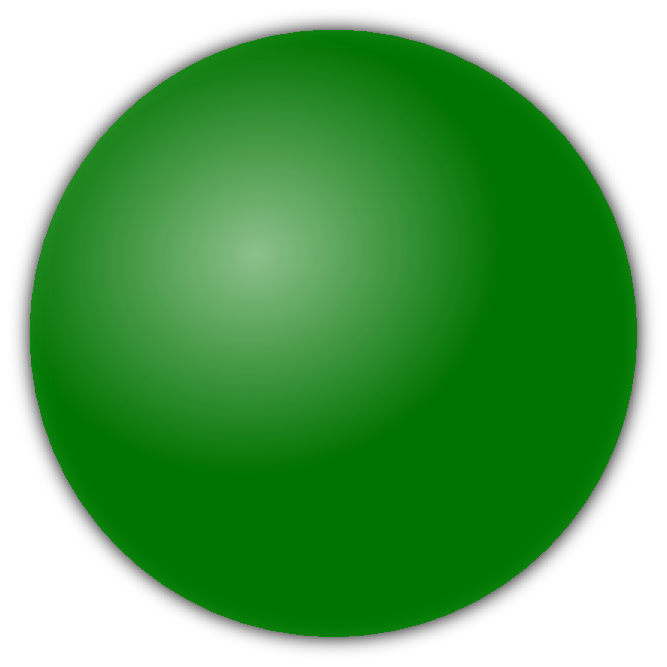
\includegraphics[scale=.4]{Pict/Sphere.pdf}  & 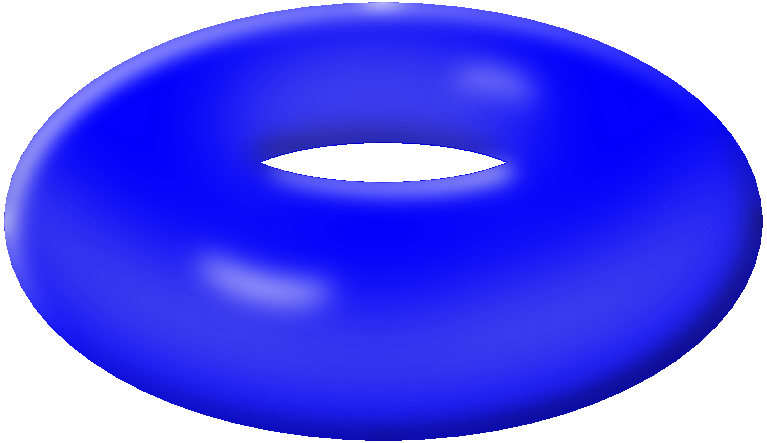
\includegraphics[scale=.4]{Pict/Torus.pdf}
  \end{tabular}
\end{center}
%% \begin{figure}[H]
%%   \begin{center}
%%      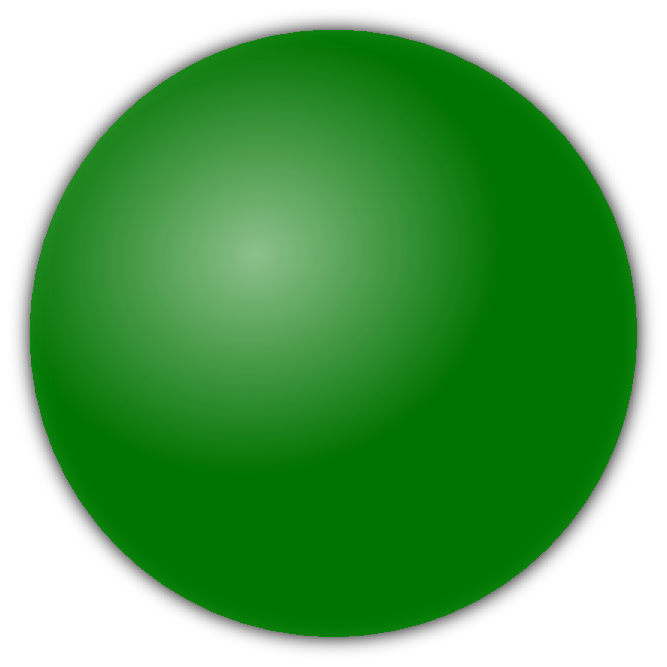
\includegraphics[scale=.4]{Pict/Sphere.pdf} 
%%      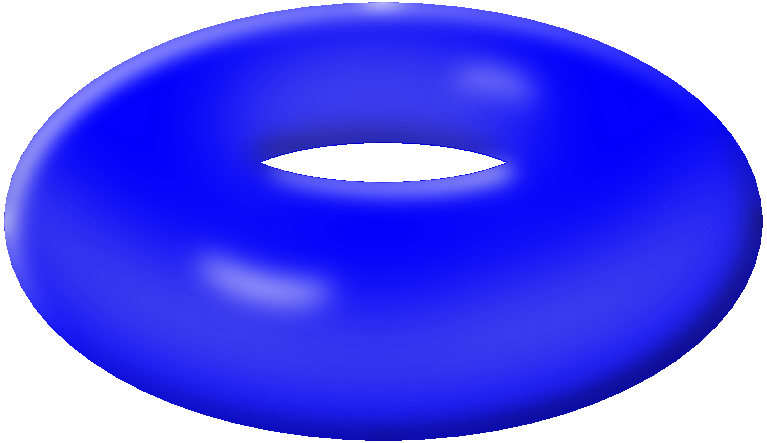
\includegraphics[scale=.4]{Pict/Torus.pdf}
%%   \end{center}
%%   \caption{Examples of manifolds}
%% \end{figure}


More illustrative is an example of a non-manifold, such as the body of a cone. A cone is not a manifold because the neighbourhood of the apex looks not line $\R^2$.
\begin{center}
  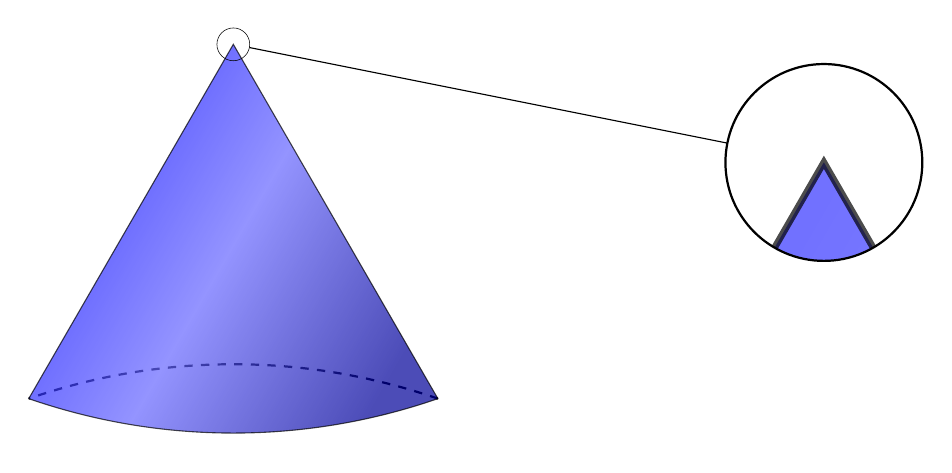
\begin{tikzpicture}[scale=1.5,
      spy using outlines={circle, magnification=6, size=2.5cm,connect spies}] 

    \pgfmathsetmacro{\a}{3}
    \pgfmathsetmacro{\b}{5}
    \pgfmathsetmacro{\th}{30}
    \pgfmathsetmacro{\ph}{atan(\a * tan(\th) / \b)}
    \pgfmathsetmacro{\r}{\a * tan(\th)}
    \pgfmathsetmacro{\h}{sqrt(\a*\a +\r*\r)}
    \pgfmathsetmacro{\H}{sqrt(\b*\b +\r*\r)}

    \coordinate (O) at (0,0);
    \coordinate (X) at (0,{\b-\a});

    \draw[thick,dashed] (X)  +(270+\th:\h) arc (90-\ph:90+\ph:\H);
    \shadedraw[left color=blue, right color= blue!60!black, middle color=blue!60!white, shading angle={90-\th}, opacity=.7] (X) -- +(270-\th:\h) arc (270-\ph:270+\ph:\H) --cycle;
    

    \spy on (X) in node at (5,1);
  \end{tikzpicture}
\end{center}

\section{Geometrical Objects on Manifolds}

One knows how to define 

\subsection{Vectors}

\subsection{One-Forms}

\subsection{Tensors}

\begin{Ebox}
  How do the components of $T$ transform? Where 
  \begin{align}
    T= T^{a_1\cdots a_p}{}_{b_1\cdots b_q} \partial_{a_1}\otimes\partial_{a_p}\otimes dx^{b_1}\otimes dx^{b_q}.
  \end{align}
\end{Ebox}

\section{Induced Maps and Submanifolds}

\subsection{Differential Map}

\subsection{Pullback Map}

\begin{Ebox}
  Let $M$, $N$ and $P$ be manifolds, and $ f:M\to N$, $g:N\to P$,  be maps between manifolds. 

  Show
  \begin{align*}
    (g\circ f)_* &= g_*\circ f_*\\
    (g\circ f)^* &= g^*\circ f^*
  \end{align*}
\end{Ebox}

\subsection{Submanifolds}

\section{Flows and Lie Derivative}

\begin{Ebox}
  For the example with $X=x\partial_y -y\partial_x$, show explicitly that 
  \begin{align}
    \sigma_t\circ \sigma_s = \sigma_{t+s}.
  \end{align}
\end{Ebox}


\begin{Ebox}
  Find the flow generated by
  \begin{align}
    X = x\partial_y +y\partial_x.
  \end{align}
\end{Ebox}

\begin{Ebox}
  \begin{itemize}
  \item Let $X$ and $Y$ be vector fields on $M$ and $f:M\to\R$ a function.
    \begin{itemize}
    \item Calculate $\Li_{X}f$.
    \item Calculate $\Li_{fX}Y$.
    \item Calculate $\Li_{X}fY$.
    \end{itemize}
  \item  Let $X$ and $Y$ be vector fields on $M$ and $f:M\to N$ a map between manifolds. Show that
    \begin{align}
      f_*\comm{X}{Y} =\comm{f_*X}{f_*Y}.
    \end{align}
  \item Let $\omega\in\Lambda^1(M)$ be a one-form on $M$. Calculate
    \begin{align}
      \Li_X \omega
    \end{align}
  \end{itemize}
\end{Ebox}

%%%%%%%%%%%%%%%%%% DIFFERENTIAL FORMS
\chapter{Exterior Calculus}

\section{Differential Forms}

\begin{Def}[Differential Forms]
  A {\sc Differential Form} of order $p$, or $p$-form, is a totally antisymmetric tensor of type $\binom{0}{p}$.
\end{Def}

Since differential form are tensor, the basis could be the same than for tensors, i.e.,
\begin{align*}
  \set{\pa{\mu}},\set{\pa{\mu}\otimes\pa{\nu}},\set{\pa{\mu}\otimes\pa{\nu}\otimes\pa{\lambda}},\cdots,
\end{align*}
however, since forms are totally antisymmetric, it is more appealing to define an antisymmetric product of the basis. This new product is called ``wedge'' product ($\w$), and is defined by
\begin{align}
  \df\, x^\mu\w\df\, x^\nu &= \df\, x^\mu\otimes\df\, x^\nu-\df\, x^\nu\otimes \df\, x^\mu\\
 &\vdots\\
  \df\, x^{\mu_1}\w\cdots\w\df\, x^{\mu_p}&= \sum_{\text{perm.}}(-1)^{\abs{\sigma}}\df\, x^{\sigma(\mu_1)}\otimes\cdots\otimes\df\, x^{\sigma(\mu_p)}
\end{align}

The vector space of differential forms of order $p$ on a manifold $M$ is denoted by $\Omega^p(M)$ or $\Lambda^p(M)$. Moreover, if $\dim(M)=m$, then
\begin{align}
  \dim\(\Lambda^p(M)\)=\binom{m}{p} =\frac{m!}{p!(m-p)!}.
\end{align}

\begin{infobox}
  In general $\Lambda^p(M)\subset \otimes^p T^*M$.
\end{infobox}

\subsection[Exterior Product]{Exterior Product (or wedge product)}

The exterior product is a map 
\begin{align}
  \w:\Lambda^p(M)\times\Lambda^q(M) \to \Lambda^{p+q}(M)
\end{align}
defined by
\begin{align}
  (\omega\w\xi)\(V_1,\cdots,V_{p+q}\) = \frac{1}{p!q!}\sum_{\text{perm.}}(-1)^{\abs{\sigma}}\omega\(V_{\sigma(1)},\cdot,V_{\sigma(p)}\)\xi\(V_{\sigma(p+1)},\cdot,V_{\sigma(p+q)}\)
\end{align}

This exterior product endows an algebra structure to 
\begin{align}
  \Lambda^\bullet(M) \equiv \Lambda^0(M)\oplus\Lambda^1(M)\oplus\cdots\oplus \Lambda^m(M).
\end{align}
Clearly,
\begin{align}
  \dim\(\Lambda^\bullet(M)\) = 2^m.
\end{align}

\subsection{Exterior Derivative}

As stated previously, although the derivative transforms like a 1-form, the derivative of a tensor is not necessarily a tensor. However, it is possible to define a ``covariant'' derivative which maps tensors into tensors.

In the same way, one defines an exterior derivative which maps $p$-forms into $(p+1)$-forms,
\begin{align}
  \df\, : \Lambda^p(M)\to\lambda^{p+1}(M),
\end{align}
defined as follows. Let $\omega$ be a differential $p$-form on $M$, then
\begin{align}
  \df\,\omega\(X_1,\cdots,X_{p+1}\) &= \sum_{i=1}^p (-1)^{i+1}X_i\[\omega\(X_1,\cdots,\hat{X}_i,\cdots,X_{p+1}\)\]\\
  &\phantom{ ==}\sum_{i<j} (-1)^{i+j}\omega\(\comm{X_i}{X_j},X_1,\cdots,\hat{X}_i,\cdots\hat{X}_i,\cdots,X_{p+1}\).\notag
\end{align}

\begin{Ebox}
  \begin{itemize}
  \item Show by explicit calculation that
    \begin{align}
      \df\,\omega_{(1)}(X,Y) = X[\omega(Y)]-Y[\omega(X)]-\omega(\comm{X}{Y}).
    \end{align}
  \item Show that if $\omega$ is a differential $p$-form with components
    \begin{align}
      \omega = \frac{1}{p!}\omega_{\mu_1\cdots\mu_p}\;\df\, x^{\mu_1}\w\cdots\w\df\, x^{\mu_p},
    \end{align}
    then its exterior derivative yields,
    \begin{align}
      \df\,\omega = \frac{1}{p!}\pa{\nu}\omega_{\mu_1\cdots\mu_p}\;\df\, x^\nu\w\df\, x^{\mu_1}\w\cdots\w\df\, x^{\mu_p}.
    \end{align}
  \end{itemize}
\end{Ebox}


It follows from the definition of the exterior derivative, that the double action of $\df\,$ vanishes, i.e., $\df\,^2=0$. This property is known as {\bf nilpotency}.





\begin{WEbox}[frametitle={Differential Forms in $\R^3$},
  frametitlerule=true,
  frametitlealignment=\centering,
  frametitleaboveskip=10pt,]
  In three dimensions the maximum order of a differential form is 3. Therefore, the complete set of forms on $\R^3$ is given by
  \begin{align*}
    \Lambda^0(\R^3) &=\F(\R^3), & \Lambda^1(\R^3) &= T^*\R^3\simeq \R^3,\notag\\
    \Lambda^2(\R^3) &= T^*\R^3\w T^*\R^3\simeq \R^3, & \Lambda^3(\R^3) &=T^*\R^3\w T^*\R^3\w T^*\R^3\simeq\F(\R^3).
  \end{align*}
  
  Let $f\in\Lambda^0(\R^3) $, then the exterior derivative of $f$ yields
  \begin{align}
    \df\, f= \frac{\partial f}{\partial x}\df\, x +\frac{\partial f}{\partial y}\df\, y +\frac{\partial f}{\partial z}\df\, z,
  \end{align}
  which is the equivalent of the gradient operation.
  
  Let $\omega\in \Lambda^1(\R^3)$ with components $\omega = \omega_x\df\, x+\omega_y\df\, y+\omega_z\df\, z$, then its exterior derivative yields,
  \begin{align}
    \df\,\omega &= \(\partial_x\omega_y-\partial_y\omega_x\)\df\, x\w\df\, y +\(\partial_y\omega_z-\partial_z\omega_y\)\df\, y\w\df\, z\notag\\
    &\phantom{==}+\(\partial_z\omega_x-\partial_x\omega_z\)\df\, z\w\df\, x, 
  \end{align}
  which is the equivalent of the curl of $\omega$.

  Let $\omega\in \Lambda^2(\R^3)$ with components $\omega = \omega_{xy}\df\, x\w\df\, y+\omega_{yz}\df\, y\w\df\, z+\omega_{zx}\df\, z\w\df\, x$, then its exterior derivative yields,
  \begin{align}
    \df\, \omega = \(\partial_x\omega_{yz}+\partial_y\omega_{zx}+\partial_z\omega_{xy}\)\df\, x\w\df\, y\w \df\, z,
  \end{align}
  which is the equivalent of the divergence of $\omega$.

  Finally, for $\omega\in\Lambda^3(\R^3)$, then $\df\,\omega=0$ due to the nilpotency of $\df\,$.


  Now, if one would like to compare with some differential properties on vector calculus, from the nilpotence of $\df\,$, it follows that
  \begin{align}
    \df\,(\df\, f) =0\quad&\Rightarrow \quad \vec{\nabla}\times \vec{\nabla}f =0,\\
    \df\,\(\df\,\omega_{(1)}\)=0 \quad&\Rightarrow\quad  \vec{\nabla}\cdot\( \vec{\nabla}\times \vec{\omega}\)=0.
  \end{align}
\end{WEbox}


\subsection{The Pullback}

A map $f:M\to N$ induces the pullback
\begin{align}
  f^*:T^*_{f(p)}N\to T^*_pM,
\end{align}
which is extended naturally to type $\binom{0}{p}$-tensors (and to differential $p$-forms),
\begin{align}
  (f^*\omega)(V_1,\cdots,V_p) =\omega(f_*V_1,\cdots,f_*V_p).
\end{align}

\begin{Ebox}
  \begin{itemize}
  \item Show that
    \begin{align}
      f^*\(\df\,\omega\) =\df\,\(f^*\omega\).
    \end{align}
    \item Show that
    \begin{align}
      f^*\(\omega\w\xi\) = f^*\omega\w f^*\xi.
    \end{align}
  \end{itemize}
\end{Ebox}


\begin{WEbox}[frametitle={Cohomology},
  frametitlerule=true,
  frametitlealignment=\centering,
  frametitleaboveskip=10pt,]
  The exterior derivative operator induces a sequence, {\it a.k.a.} a complex,
  \begin{align}
    0\stackrel{~i~}{\hookrightarrow }\Lambda^0(M) \xrightarrow{~\df\,~}\Lambda^1(M) \xrightarrow{~\df\,~}\cdots\xrightarrow{~\df\,~} \Lambda^{m-1}(M) \xrightarrow{~\df\,~}\Lambda^m(M) \xrightarrow{~\df\,~} 0,
  \end{align}
  called the {\bf de Rham complex}.

  Defining,
  \begin{itemize}
  \item A form, $\omega$, is said to be closed if $\df\,\omega =0$.
  \item A form, $\omega$, is said to be exact if $\omega =\df\,\xi$.
  \end{itemize}

  Due to the nilpotency of $\df\,$, it follows that,
  {\small
  \begin{align*}
    \Im\(\df\,:C^\infty\(\Lambda^{p-1}(M)\)\to C^\infty\(\Lambda^{p}(M)\)\)\subset\Ker\(\df\,:C^\infty\(\Lambda^{p}(M)\)\to C^\infty\(\Lambda^{p+1}(M)\) \).
  \end{align*}
  }

  Therefore, the {\bf $\mathbf{p}$-th de Rham Cohomology group}, $H^p(M)$, is defined by
  \begin{align*}
    H^p(M)\equiv \frac{\Ker\(\df\,:C^\infty\(\Lambda^{p}(M)\)\to C^\infty\(\Lambda^{p+1}(M)\) \)}{\Im\(\df\,:C^\infty\(\Lambda^{p-1}(M)\)\to C^\infty\(\Lambda^{p}(M)\)\)}.
  \end{align*}
\end{WEbox}


\subsection{Interior Product and Lie Derivative}

The interior product is  a map
\begin{align}
  i:TM\times \Lambda^p(M)\to \Lambda^{p-1}(M),
\end{align}
or usually denoted
\begin{align}
  i_X:\Lambda^p(M)\to \Lambda^{p-1}(M),
\end{align}
defined by
\begin{align}
  i_X\omega(V_1,\cdots,V_{p-1})=\omega(X,V_1,\cdots,V_{p-1}).
\end{align}
In components it can be written as
\begin{align}
  i_X\omega &= \frac{1}{(p-1)!}X^\nu \omega_{\nu \mu_2 \cdots\mu_{p}}\;\df\, x^{\mu_2}\w\cdots\w\df\, x^{\mu_p}\\
  &= \frac{1}{p!}\sum_{s=1}^p X^{\mu_s} \omega_{\mu_1 \cdots\mu_s \cdots \mu_{p}}\;\df\, x^{\mu_2}\w\cdots\w\widehat{\df\, x}^{\mu_s}\w\cdots\w\df\, x^{\mu_p}.\notag
\end{align}


Using the exterior derivative and the interior product, one can construct the operator $\df\, i_x+i_X \df\,$. This operator can be applied to 1-forms,
\begin{align}
  \(\df\, i_x+i_X \df\,\)\omega &=\df\,(X^\mu\omega_\mu) +i_x\(\pa{\mu}\omega_\nu \df\, x^\mu\w\df\, x^\nu\)\notag\\
  &=\(\pa{\nu}X^\mu\)\omega_\mu\df\, x^\nu +X^\mu\(\pa{\nu}\omega_\mu\)\df\, x^\nu +X^\mu\(\pa{\mu}\omega_\nu-\pa{\nu}\omega_\mu\)\df\, x^\nu\notag\\
  &=\[\omega(\pa{\nu}X^\mu)+X^\mu(\pa{\mu}\omega_\nu)\]\df\, x^\nu,
\end{align}
which is nothing but the Lie derivative of a differential 1-form,
\begin{align}
  \Li_X\omega = \(\df\, i_X + i_X \df\,\)\omega.
\end{align}
The above expression is general for differential forms of any order.

The interior product and the Lie derivative satisfy
\begin{align}
  i_X\(\omega\w\eta\)&=\(i_X\omega\) \w \eta+(-1)^{\abs{\omega}}\omega \w \(i_X\eta\)\\
  i_X^2&=0\\
  \Li_X i_X\omega &= i_X\Li_X\omega.
\end{align}


\begin{WEbox}[frametitle={Geometry of Classical Mechanics},
  frametitlerule=true,
  frametitlealignment=\centering,
  frametitleaboveskip=10pt,]
  Let $M$ be a $m$-dimensional manifold, and $\Phi^m\equiv T^*M$ be its cotangent bundle (or {\bf phase space}). A {\bf Hamiltonian} on $M$ is a map $\Ha:\Phi^m\to \R$.

  Let $\set{q^\mu,p_\mu}$, with $\mu=1...m$, be  the coordinates on $\Phi^m$. One might define a symplectic form on $\Phi^m$ by
  \begin{align*}
    \Lambda^2\(\Phi^m\)\ni \omega = \df\, p_\mu\w\df\, q^\mu,
  \end{align*}
  and a 1-form $\theta=q^\mu \df\, p_\mu\in \Lambda^1\(\Phi^m\)$, s.t. $\omega=-\df\,\theta$.
  
  Given a function $f:\Phi^m\to \R$. one might define the {\sc Hamiltonian Vector Field}
  \begin{align*}
    X_f = \pder{f}{p_\mu}\pder{}{q^\mu} -\pder{f}{q^\mu}\pder{}{p_\mu}.
  \end{align*}
  Then,
  \begin{align*}
    i_{X_f}\omega =-\pder{f}{q^\mu}\df\, q^\mu -\pder{f}{p_\mu}\df\, p_\mu = -\df\, f.
  \end{align*}

  The Hamilton equations,
  \begin{align*}
    \dot{q}^\mu =\pder{\Ha}{p_\mu},\quad \dot{p}_\mu =-\pder{\Ha}{q^\mu},
  \end{align*}
  can be written as
  \begin{align*}
    i_{X_\Ha}\omega = -\pder{\Ha}{q^\mu}\df\, q^\mu -\pder{\Ha}{p_\mu}\df\, p_\mu = -\df\,\Ha,
  \end{align*}
  where the identity
  \begin{align*}
    X_\Ha &=\pder{\Ha}{p_\mu}\pder{}{q^\mu} -\pder{\Ha}{q^\mu}\pder{}{p_\mu}\\
    &= \dot{q}^\mu\pder{}{q^\mu} +\dot{p}_\mu\pder{}{p_\mu}\\
    &= \der{}{t},
  \end{align*}
  has been used.

  Also, the action of two interior products on $\omega$ yields the Poisson bracket,
  \begin{align*}
    i_{X_f}\(i_{X_g}\omega\) &=-i_{X_f}(\df\, g) = -i_{X_f}\(\pder{g}{q^\mu}\df\, q^\mu +\pder{g}{p_\mu}\df\, p_\mu\)\\
    &= -\pder{f}{p_\mu}\pder{g}{q^\mu}+\pder{f}{q^\mu}\pder{g}{p_\mu}\\
    &=\acomm{f}{g}_{P.B.}.
  \end{align*}
\end{WEbox}

\begin{WEbox}[frametitle={Gauge Theory (Abelian)},
  frametitlerule=true,
  frametitlealignment=\centering,
  frametitleaboveskip=10pt,]
  Let $M$ be a four-dimensional, flat, Lorentzian spacetime endowed with a Minkowski metric, $\eta=\diag(-1,1,1,1)$, and $A_\mu = (-\phi,\vec{A})$ be a four-vector on $T^*M$. One can construct the 1-form 
  \begin{align}
    A = -\phi\df\, t +A_i\df\, x^i.
  \end{align}

  Define the 2-form, $F$ as the exterior derivative of $A$,
  \begin{align}
    F &= \df\, A\\
    &= -\partial_i\phi\;\df\, x^i\w\df\, t +\partial_t A_i\;\df\, t\w\df\, x^i + \partial_i A_j\;\df\, x^i\w\df\, x^j\\
    &= \(\partial_i\phi+\partial_t A_i\)\;\df\, t\w\df\, x^i+ \partial_i A_j\;\df\, x^i\w\df\, x^j\\
    &= -\df\, t\w \mathbf{E}_{(1)} +\mathbf{B}_{(2)},
  \end{align}
  where the differential forms $\mathbf{E}$ and $\mathbf{B}$ are the associated to the electric and magnetic field.
  
  Now, the nilpotency of $\df\,$ implies that,
  \begin{align}
    \df\, F = \df\,\df\, A =0,
  \end{align}
  while on the other hand, 
  \begin{align}
    \df\, F = \df\, t\w \df\,_s\mathbf{E}_{(1)} +\df\,_t\mathbf{B}_{(2)}+\df\,_s\mathbf{B}_{(2)},\label{MaxdF}
  \end{align}
  where $\df\,_t$ and $\df\,_s$ are the exterior derivative on the time and space respectively.
  
  Since the basis elements $\df\, t$ and $\df\, x^i$ are linearly independent, it follows that components containing projections along the time are independent of those lying only on the space. Thus, Eq. (\ref{MaxdF}), decompose into two independent equations,
  \begin{align}
    \partial_t \vec{B} +\vec{\nabla}\cdot\vec{E} &=0,\notag\\
    \vec{\nabla}\cdot\vec{B}&=0,\label{MaxBianchi}
  \end{align}
  where the relation between the exterior derivative on forms and the vector calculus have been used. The Eq. (\ref{MaxBianchi}) are known as the Maxwell equations coming from the Bianchi identity.

  When a change can be made to the geometrical object, $A$ in this case, and the physical fields (what can be measured) do not vary, $\vec{E}$ and $\vec{B}$, the theory is said to posses a  {\bf gauge  invariance}.

  The electromagnetic theory is a gauge theory. Note that the electric and magnetic fields enters through $F$, not through $A$. Thus, if one changes $A\mapsto A+\df\, f$, the $F$ field do not changes,
  \begin{align}
    F\to F' = \df\, A' = \df\,\( A+\df\, f\) = \df\, A = F.
  \end{align}

  In order to conclude, it is worth to remark that the physical observables of the electromagnetic theory, $\vec{E}$ and $\vec{B}$, lie in a close form, $F$, but are defined up to a gauge transformation, i.e., $A$ is unique up to an exact form. Therefore, the physical states live in the second cohomological group of the Minkowski space, $H^2\(\R^{1,3}\)$.
\end{WEbox}


\section{Lie Groups and Lie Algebras}

\subsection{Lie Groups}

\begin{Def}[Group]
  A {\sc Group} $G$ is a set of elements, $\{g\}$, together with an operator, $\cdot: G\to G$, satisfying
  \begin{enumerate}
  \item Exists an unique identity element, $e$, s.t. $e\cdot g=g\cdot e =g$ for all $g\in G$.
  \item For every pair $g_1,g_2\in G$, the product $g_1\cdot g_2\equiv g_3$ belongs to $G$.
  \item Associativity: $g_1\cdot(g_2\cdot g_3)= (g_1\cdot g_2)\cdot g_3$, for all $g_1,g_2,g_3\in G$.
  \item Exists an inverse $g^{-1}\in G\; \forall g\in G$ s.t. $g\cdot g^{-1}=g^{-1}\cdot g=e$.
  \end{enumerate}
\end{Def}



%%%%%%%%%%%%%%%%%% BUNDLES AND CONNECTION

\chapter{Bundles and Connections}

So far, tangent and cotangent bundles have been considered, and other generalisations have been slightly appearing.

Instead of attacking the problem formally, in the following, a heuristic introduction to more general bundles is shown, and also the definition of connections on these bundles.

\section{Fibre Bundles}

A \emph{\idx{Bundle}} is a geometric structure composed by two manifolds $E$ (the bundle) and $M$ (the base)\footnote{In some sense the base manifold is a ``piece'' of the bundle, i.e., $M \subset E$.} together with a projection map $\pi: E \to M$. If $U \subset M$, then locally, $E \simeq U \times F$, where $F$ is a manifold called the fibre of $E$. 

\subsubsection*{Examples}
\begin{itemize}
\item A cylinder is a bundle $E$ with base manifold $M = \R$ and fibre $F = S^1$, s.t. $\pi: \R \times S^1 \to \R$.
  
  In this case, $E = M \times F$ globally, then the bundle is called \emph{Trivial}\index{Bundle!trivial}.
\item If one takes an interval $I \subset \R$, the ``finite'' cylinder is a trivial bundle $E = I \times S^1$ or $E = S^1 \times I$.
\item The simplest non-trivial bundle is a M\"obius strip, which is a bundle $E$ locally homeomorphic to $S^1 \times I$, but is not globally $S^1 \times I$ because there is a ``twist'' (a bit more formally there is a $Z_2$-action on the fibre).
  \begin{center}
    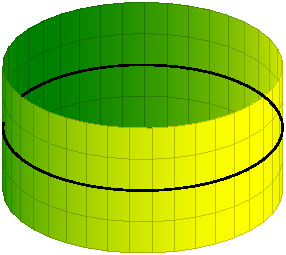
\includegraphics{Pict/tikz-cylinder.pdf}
    \hspace{5em}
    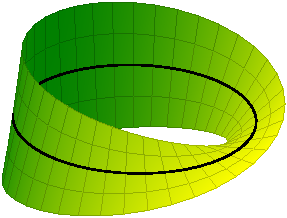
\includegraphics{Pict/tikz-moebius.pdf}
  \end{center}
\item  A 2-torus $T^2$ is a trivial bundle with base manifold $M = S^1$ and fibre $F = S^1$.
\end{itemize}

In essence there are three types of bundles:
\begin{description}
\item [Fibre Bundle]\index{Bundle!fibre} is a general bundle structure, i.e., a manifold which locally looks like a product of a base manifold and the fibre.
\item [Vector Bundle]\index{Bundle!vector} A fibre bundle whose fibre is a vector space.
\item [Principal Bundle]\index{Bundle!principal} A fibre bundle whose fibre is a manifold with group structure, i.e., the fibre is a Lie group manifold.
\end{description}

\subsection{Sections on Bundles}

A \idx{Section}, $\psi$, on a bundle $E \xrightarrow{\pi} M$ is a smooth map from the base manifold to the bundle,
\begin{align}
  \psi: M \to E,  
\end{align}
such that $\pi \circ \psi = \id_M$.

Sections are one important object for physicist, because they represent the physical fields of a theory.

\subsection{More About Principal Bundles}

As stated before, principal bundles are fibre bundles whose fibres are a Lie Group. Therefore, there is an action of $G$ on $F$. They are the natural framework for the study of Gauge Theories.

\subsubsection*{Associated Bundles}

The associated bundles are constructed from  principal bundles. Let $P(M,G)$ be a principal bundle, with fibre $F$ admitting and action of the Lie group $G$.

Given a pair $(u,f)$ on $P \times F$, a bundle $\(P \times F\)/G$ can be construct by identifying points related by the action of the group $G$, 
\begin{align}
  (u,f)\sim \( u g, g^{-1} f \).
\end{align}
This construction is known as \emph{associated bundle}\index{Bundle!associated}.

More generally, the fibre can admit the action of a representation $\rho$ of $G$. In this case, the associated bundle $\(P \times_\rho F\)/G$ is constructed through,
\begin{align}
  (u,f) \sim \( u g, \rho\(g^{-1}\) f \).
\end{align}


\section{Connections on the Tangent Bundle}

A connection on the tangent bundle is an application $\nabla: TM \times TM \to TM$, defined by
\begin{align}
  \nabla: (X,Y) \to \nabla_X Y,
\end{align}
satisfying 
\begin{align}
  \nabla_{f X} Y &=f \nabla_X Y\\
  \nabla_X f Y &= f\nabla_X Y + Y \cdot X[f],\\
  \nabla_{X + Y} Z &= \nabla_X Z + \nabla_Y Z.
\end{align}

On a vector basis, 
\begin{align}
  \nabla_{\partial_i} \partial_j \equiv \nabla_i \partial_j = \conn{i}{k}{j} \pa{k},
\end{align}
then, in components
\begin{align}
  \nab{i} Y=\(\pa{i} Y^j + \conn{i}{j}{k} Y^k\) \pa{j}.
\end{align}
In physics, the term between the brackets is called the covariant derivative of a vector.


\begin{infobox}[frametitle={General Connections}]
  In a general bundle $E$, the connections are applications
  \begin{align*}
    \nabla: TM \otimes \mathcal{E} \to \mathcal{E},
  \end{align*}
  where $\mathcal{E}$ is the space of sections on the bundle $E$.
\end{infobox}

\section{Parallel Transport and Geodesic}

Let $V$ be a tangent vector to a curve, i.e., 
\begin{align}
  V = \der{x^\mu}{ t} \(c(t)\) \;\pa{\mu}\bigr|_{c(t)},
\end{align}
then $X\in TM$ is said to be parallel transported\index{Parallel transport} along $c(t)$ if
\begin{align}
  \nabla_V X =0\quad \forall\;t\in I.
\end{align}

If the tangent vector to a curve ($V$) satisfies the parallel transport condition,
\begin{align}
  \nabla_V V =0,
\end{align}
then the curve $c(t)$ is called a \emph{\idx{Geodesic}}.

\begin{Ebox}
  \begin{itemize}
  \item Use that
    \begin{align*}
      \nab{i} \pa{j} &= \conn{i}{k}{j} \pa{k}\\
      \nab{i}' \pa{j}' &= \(\Ga_{i}'\)^{k}{}_{j} \pa{k}',
    \end{align*}
    to find the transformation rule of $\Ga$'s.
  \item Find the action of $\nabla$ on 1-forms and rank two tensors.
  \item Write in coordinates the condition of parallel transport and geodesic curve.
  \end{itemize}
\end{Ebox}


\section{Torsion and Curvature}

\begin{align}
  T(X,Y) &= \nab{X}Y-\nab{Y}X-\comm{X}{Y}\\
  R(X,Y,Z) &= \nab{X}\nab{Y}Z -\nab{Y}\nab{X}Z -\nab{\comm{X}{Y}}Z.
\end{align}

\begin{Ebox}
  \begin{itemize}
  \item Find coordinate expressions for $T(X,Y)$ and $R(X,Y,Z)$.
  \item Show that they are multilinear objects, i.e., they are tensors.
  \end{itemize}
\end{Ebox}
\bigskip
\begin{infobox}[frametitle={NOTE}]
  In general the concept of curvature can be extended to sections on a bundle, where 
  \begin{align*}
    \nabla: TM \otimes \mathcal{E} \to \mathcal{E},
  \end{align*}
  while the torsion cannot, since $X$ and $Y$ are necessarily the same kind of object.
\end{infobox}



%%%%%%%%%%%%%%%%%% RIEMANNIAN MANIFOLDS

\chapter{Riemannian Manifolds}

\section{The metric}

\begin{Def}[Riemannian Metric]
  Let $M$ be a differential manifold. A \emph{\idx{Riemannian metric}}, $g$ on $M$ is a symmetric, non-degenerated $\binom{0}{2}$-tensor, i.e.,
  \begin{align}
    g(X,Y) &= g(Y,X)\\
    g(X,X) &= 0 \quad \text{iff } X = 0.
    \label{riem-cond}
  \end{align}
\end{Def}

If the metric satisfies the condition
\begin{align}
  g(X,Y) = 0 \quad \forall X \, \Rightarrow \, Y = 0.
  \label{sriem-cond}
\end{align}
instead of Eq.~\eqref{riem-cond}, the metric is said to be semi-Riemannian\index{Semi-Riemaniann metric}.

Given a set of coordinated on $M$, the metric is expressed as 
\begin{align}
  g_p = g_{\mu\nu}(p) \, \de{x}^\mu \otimes \de{x}^\nu,
\end{align}
with
\begin{align}
  g_{\mu\nu}(p) = g_p\(\partial_\mu, \partial_\nu\).
\end{align}

The metric can be seen as a map
\begin{equation}
  \begin{split}
    g_p: T_pM \times T_pM &\to \R,\\
    g_p: T_pM &\to T^*_pM,
  \end{split}
\end{equation}
and its inverse, $g^{-1}$, similarly yields
\begin{equation}
  \begin{split}
    g^{-1}_p: T^*_pM \times T^*_pM &\to \R,\\
    g^{-1}_p: T^*_pM &\to T_pM.
  \end{split}
\end{equation}

In index notation, the inverse metric is denoted with upper indices, i.e., 
\begin{align}
  \(g^{-1}\)_{\mu\nu} = g^{\mu\nu},
\end{align}
such that,
\begin{align}
  g_{\mu\nu}g^{\nu\lambda} = \delta_\mu^\lambda.
\end{align}

One might consider metrics compatible with the connection, 
\begin{align}
  \nabla_X g = 0, \quad \forall \, X \in TM.
\end{align}

\begin{Ebox}
  Use the \emph{metric compatibility} condition, to find a expression for the (general) connection in terms of the metric and the skew-symmetric part of the $\Gamma$'s.
\end{Ebox}


\section{Metric Structure and Impact on Differential Forms}

It has been pointed out before that the only geometrical object one can integrate on an orientable $m$-dimensional manifold is a $m$-form. However, on Riemannian manifolds, were the metric defines a volume form, one in accustomed to integrate functions.

The link between the two notions is made by defining a new sort of differential operator, called the \emph{\idx{Hodge star}}, as follows
\begin{align}
  *: C^\infty \(\Lambda^p(M)\) \to C^\infty \(\Lambda^{m-p}(M)\)
\end{align}
such that, for $\alpha,\beta \in C^\infty \(\Lambda^p(M)\)$,
\begin{align}
  \bk{\alpha}{\beta} = \int \alpha \we * \beta
  = \int_M (\alpha,\beta) \de{V}_g
  = \int\,\dn{m}{x}\sqrt{g}\,\alpha_{a_1\cdots a_p}\beta_{b_1\cdots b_p}g^{a_1 b_1}\cdots g^{a_p b_p}.
  \label{HodgeDef}
\end{align}


\begin{Ebox}
  \begin{itemize}
  \item Use Eq.~\eqref{HodgeDef} to find the action of $*$ on the basis of differential forms.
  \item Show that the double action of the Hodge star is proportional to the unit, i.e.,
    \begin{equation*}
      *^2 \alpha \simeq \alpha
    \end{equation*}
  \end{itemize}
\end{Ebox}


Using this, a formal  dual of the differential operator $\dfd\,$ can be defined,
\begin{align}
  \dfd\,: \Lambda^p(M) \to \Lambda^{p-1}(M),
\end{align}
such that (on compact manifolds)
\begin{align}
  \bk{\dfd\, \alpha_{(p+1)}}{\beta_{(p)}}=\bk{\alpha_{(p+1)}}{\df\,\beta_{(p)}}.
\end{align}
The operator $\dfd\,$ is called co-differential, and it is nilpotent as its partner $\df\,$, i.e., $\df\,^2 ={\dfd\,}^2=0$. Also, a differential form is said to be co-closed is $\dfd\,\alpha=0$ and co-exact if $\alpha=\dfd\,\beta$, thus, $\dfd\,$ defines a complex, and a homology.


\begin{Ebox}
  Use the symmetric properties of the product of forms and the ``idempotency'' of the Hodge star operation, to find an expression of the co-differential operator in terms of $\df\,$ and $*$.
\end{Ebox}



Using the differential and co-differential operators on forms, the Laplacian on differential forms can be defined by,
\begin{align}
  \Delta:C^\infty\(\Lambda^p(M)\) &\to C^\infty\(\Lambda^p(M)\)\\
  \Delta&= \df\dfd\,+\dfd\,\df
\end{align}
A form satisfying $\Delta\alpha=0$ is said to be an {\bf Harmonic Form}.

\begin{Thm}
  On a compact, oriented Riemannian manifold one can define the space of harmonic forms by
  \begin{align}
    \Ha^k = \Ker\(\Delta:C^\infty\(\Lambda^p(M)\) \to C^\infty\(\Lambda^p(M)\)\),
  \end{align}
  then it follows that for every $\alpha\in \Ha^k$, $\alpha$ is closed and co-closed. 
\end{Thm}
\begin{proof}
  Since $\Delta\alpha=0$, then
  \begin{align}
    0=\bk{\alpha}{\Delta\alpha}&=\bk{\alpha}{\df\dfd\,\alpha}+ \bk{\alpha}{\dfd\,\df\,\alpha}\\
    &=\bk{\dfd\,\alpha}{\dfd\,\alpha}+ \bk{\df\,\alpha}{\df\,\alpha}\\
    &= \norm{\dfd\,\alpha}^2+ \norm{\df\,\alpha}^2.
  \end{align}
  Since the sum of positive quantities vanishes, each quantity must vanish separately. Therefore,
  \begin{align}
    \df\,\alpha=\dfd\,\alpha=0.
  \end{align}
\end{proof}


\section{Defining Actions in Physics}

Now the machinery for constructing physical actions has been presented. Thus in this section, different actions will be shown.

%In the lectures a part of the Abelian gauge theories was worked out, therefore it will be presented as first example.

\subsection{Classical (non-relativistic) Point Particle}

In classical physics the observed quantities are coordinates in $\R^3$, $x^i$ with $i=1,2,3$, denoting the position of a particle, while the only parameter is the time,  $t\in \R$.

Therefore, a classical, non-relativistic, massive, point-particle is described by a map $x:\R\to\R^3$. In the language of bundles, $x$ is a section on a fibre bundle, $E\xrightarrow{~\pi~}M$, where the base manifold is the $\R$ (the time manifold), and its fibre is $\R^3$. Additionally, on the fibre an inner product is defined, $\bk{\bullet}{\bullet}$.




\subsection{Electromagnetic Action}

The electromagnetic action is a theory of a connection $\AF{1}$, with values on an Abelian gauge group ($U(1)$). The fundamental object for constructing the action is the field strength, $\FF{2}=\df\,\AF{1}$, which is gauge invariant.

Using differential forms the action is,
\begin{align}
  \int\Lag[\AF{1}] = -\frac{1}{2}\int \FF{2}\w *\FF{2}+\int \AF{1}\w*J
\end{align}


\begin{Ebox}
  \begin{itemize}
  \item Use the properties of the exterior differentiation to find the equation of motion of the field $\AF{1}$.
  \item Write the equations in components, then use the definitions of $\vec{E}$ and $\vec{B}$ to find the usual Maxwell equations.
  \item Use the nilpotence of $\df\,$ (or $\dfd\,$) to find the continuity equation of $J$.
  \item Show that the Lorentz condition $\partial_\mu A^\mu$ is expressed as $\df\,*\AF{1}$.
  \end{itemize}
\end{Ebox}



\subsection{Non-Abelian Gauge Theories}

In order to go beyond the Abelian gauge theories, it is useful to give geometrical interpretation to the fields.

As all of the physical theories, a gauge theory lies on a Minkowski spacetime, $M$, and the fields transform as irreps of the Lorentz group. In the case of a gauge boson,  $\AF{1}$, the field transforms under the (co)vector representation, therefore $\AF{1}$ is a section on the cotangent bundle ($T^*M$).

Additionally, the field transforms as a connection under gauge transformations of a group $G$. Then, the field is also a section of the principal bundle $P(M,G)$, specifically $\AF{1}$ is a section on the associated bundle $P(M,G)\times_{Ad_G}\mathfrak{g}$.

Since the field is not invariant, the Lagrangian density must be made invariant. Then, an inner product on $\mathfrak{g}$ should be considered, denoted $\vev{\bullet}$.

Finally, the Lagrangian density is
\begin{align}
  \Lag[\AF{1}] =-\frac{1}{2} \vev{\FF{2}\w*\FF{2}},
\end{align}
where $\FF{2}$ is the curvature of the connection $\AF{1}$, defined by the ``twisted'' exterior derivative $\df\,_{\AF{1}}= \df\, +\AF{1}$,
\begin{align}
  \FF{2}= \df\,_{\AF{1}}\AF{1}= \df\,\AF{1} +\frac{1}{2}\AF{1}\w\AF{1}
\end{align}


\begin{WEbox}[%
    frametitle={Equations of Motion for Yang-Mills Theories},
    frametitlerule=true,
    frametitlealignment=\centering,
    frametitleaboveskip=10pt,]
  In order to find the equation of motion of a Yang-Mills theory, one might use the fact that the ``twist'' derivative, $\df\,_{\AF{1}}$, acts on charged fields, then
  \begin{align*}
    \int \Lag[\AF{1}] &=-\frac{1}{2}\int \vev{\FF{2}\w*\FF{2}}\\
    &=-\frac{1}{2}\int \df\,_{\AF{1}}\vev{\AF{1}\w*\FF{2}}-\frac{1}{2}\int \vev{\AF{1}\w\df\,_{\AF{1}}*\FF{2}}\\
    &=-\frac{1}{2}\int \df\,\vev{\AF{1}\w*\FF{2}}-\frac{1}{2}\int \vev{\AF{1}\w\df\,_{\AF{1}}*\FF{2}},
  \end{align*}
  the first term vanishes for fields with compact support (or manifolds without boundaries), then, the equation of motion is 
  \begin{align*}
    \dfd\,_{\AF{1}}\FF{2} =0.
  \end{align*}
\end{WEbox}





\section{General Relativity Tensors}

The formulation of General Relativity (GR) lies on the absence of torsion, therefore the only geometrical tensor which measures the lack of Euclidean structures on $M$ is the curvature.

Roughly speaking the goal of GR is to associate the gravitational interaction to the geometrical deformation of the manifold. Therefore, one must mix objects with the geometrical information of the manifold with the object containing the matter distribution. The former is related with the Riemann tensor, while the later is the stress-energy tensor. Immediately, one notes that the rank of these tensors is not compatible, thus some arrange must be done.

Using the curvature tensor, other simplified tensors can be constructed
\begin{align}
  \Ric(X,Y) &= \bk{\df\, x^\mu}{R(\partial_\mu,Y)X}\\
  \Ri &= g^{\mu \nu}\Ric(\partial_\mu,\partial_\nu).
\end{align}
Since in most cases the stress-energy tensor is symmetric, it seems that Einstein's first proposal for the equations of gravity were
\begin{align}
  \Ri_{\mu\nu}=T_{\mu\nu},
\end{align}
but the R.H.S. of the equation was covariantly constant, while the L.H.S. was not. Thus, a covariantly constant construction made up with ``curvature'' tensors was
\begin{align}
  G_{\mu\nu} = \Ri_{\mu\nu}-\frac{1}{2}g_{\mu\nu}\Ri,
\end{align}
this tensor is known as Einstein tensor, ans the equation of gravity are written as,
\begin{align}
  G_{\mu\nu}= T_{\mu\nu}.
\end{align}
Additionally, there are spaces with ``cosmological constant'', $\Lambda$, and the Einstein's equations for this kind of spacetimes are
\begin{align}
  \Ri_{\mu\nu}-\frac{1}{2}g_{\mu\nu}\Ri + \Lambda g_{\mu\nu}= T_{\mu\nu}.
\end{align}

A manifold whose Ricci tensor is proportional to the metric is said to be an Einstein manifold,
\begin{align}
  \Ri_{\mu\nu} = \kappa g_{\mu\nu}.\label{def-const-curv}
\end{align}

Also, a manifold is said to have constant curvature if its curvature 2-form is
\begin{align}
  \Rif{ab}{} = \kappa\vif{a}\w\vif{b},
\end{align}
for a constant value $\kappa$.

\begin{Ebox}
  \begin{itemize}
  \item Show that in vacuum, i.e., $T_{\mu\nu}=0$, Einstein's equations (without cosmological constant) might be written as
    \begin{align}
      \Ri_{\mu\nu}=0.
    \end{align}
  \item Show that in general, Einstein's equations  (without cosmological constant) might be written as
    \begin{align}
      \Ri_{\mu\nu}= T_{\mu\nu}-\frac{1}{D-2}g_{\mu\nu} T,
    \end{align}
    where $T$ is the trace of the Stress-Energy tensor,  and  $D$ is the spacetime dimension. These equations are known as Einstein's equations in the form of Ricci.
  \item Derive the Einstein's equations in the form of Ricci, when the cosmological constant does not vanish.
  \end{itemize}
\end{Ebox}




%%%%%%%%%%%%%%%%%% ANOTHER LECTURE

\chapter{Cartan Calculations in (semi)Riemannian Geometry}

Before continuing, a change of notation will be made. Although this can be confusing, the previous notation is used often by mathematicians, while the following is used by physicist.

\section{Frame Fields in (semi)Riemannian Geometry}

%Before continuing, a change of notation will be made. Although this can be confusing, the previous notation is used often by mathematicians, while the following is used by physicist.

Let $M$ be a manifold, and $g$ a (semi)Riemannian metric defined on $M$. Then the line element for the metric $g$ is
\begin{align}
  \de{s}^2(g) = g_{\mu\nu} \de{x}^\mu \otimes \de{x}^\nu.
\end{align}
Nonetheless, the information about the metric structure of the manifold can be translate to the languages of frames,
\begin{equation}
  \begin{split}
    \de{s}^2(g)
    &= g_{\mu\nu} \de{x}^\mu \otimes \de{x}^\nu \\
    &= \eta_{ab} \; \vi{a}{\mu}(x) \, \vi{b}{\nu}(x) \; \de{x}^\mu \otimes \de{x}^\nu \\
    &= \eta_{ab} \; \vif{a} \otimes \vif{b}.
  \end{split}
\end{equation}
Therefore, the vielbein, $\vif{a}$, is the fields equivalent to the metric tensor. In order to complete the structure, one needs information about the transport of geometrical objects lying on bundles based on $M$. That information is encoded on the spin connection, $\spif{a}{b}$. Using these quantities one finds  the generalisation of the structure equations of Cartan,
\begin{align}
  \df \vif{a} + \spif{a}{b} \we \vif{b} &= \Tf{a},
  \label{firstSE}\\
  \df \spif{a}{c} + \spif{a}{b} \we \spif{b}{c} &= \Rif{a}{c}
  \label{secondSE}.
\end{align}
In the sense of the previous lesson, the torsion 2-form, $\Tf{a}$, and the curvature 2-form,$\Rif{a}{c}$, measure the impossibility of endow an Euclidean structure on $M$.

\subsection*{Remarks on the Structure Equations}

\begin{itemize}
\item In general relativity, the torsion vanishes. Therefore, the first Cartan's structure Eq.~\eqref{firstSE}, yields an explicit expression for the spin connection as a function of the vielbein. This is equivalent to the well-known expression of the Levi-Civita connection $\Gamma_\mu{}^\lambda{}_\nu$ as a function of the metric and its derivatives.
\item The components of the torsion and curvature 2-forms are given by
%%%%
%% Change the eq. of the torsion (to be the equiv of the curvature
%%%%
  \begin{align}
    \Tf{a} &= \frac{1}{2} \tors{\mu}{a}{\nu} \; \de{x}^\mu \we \de{x}^\nu,
    \label{def-tor-comp} \\
    %\tor_\mu{}^\lambda{}_\nu \;\df\; x^\mu\w\df\; x^\nu &= \tor_a{}^c{}_b \vin{\lambda}{c}\;\vif{a}\w\vif{b},\\
    \Rif{a}{b} &= \frac{1}{2} \Ri^a{}_{b\mu\nu} \; \de{x}^\mu \we \de{x}^\nu.
    \label{def-curv-comp}
  \end{align}
\end{itemize}

\section{Playing with the Structure Equations}

From the first S.E.
\begin{align*}
  \df \( \df \vif{a} + \spif{a}{b} \we \vif{b} \) &= \df \Tf{a} \\
  \therefore \quad
  \df \Tf{a} &= \( \df \spif{a}{b}\) \we \vif{b} - \spif{a}{b} \we \df \vif{b}  \\
  \df \Tf{a} &= \( \Rif{a}{b} - \spif{a}{c} \we \spif{c}{b}\) \we \vif{b} - \spif{a}{c} \we \df \vif{c} \\
  \df \Tf{a} &= \Rif{a}{b} \we \vif{b} - \spif{a}{c} \we \( \spif{c}{b} \we \vif{b} + \df \vif{c} \) \\
  \df \Tf{a} &= \Rif{a}{b} \we \vif{b}-\spif{a}{c} \we \Tf{c},
  %  \Rif{a}{b} \we \vif{b}&=\cdf\Tf{a}
\end{align*}
then,
\begin{align}
  \Rif{a}{b} \we \vif{b}&=\df\Tf{a}+\spif{a}{c} \we \Tf{c}.
\end{align}


From the second S.E.
\begin{align*}
  \df\(\df\spif{a}{b}+\spif{a}{c} \we \spif{c}{b}\) &= \df\Rif{a}{b}\\
  \therefore \quad
  \df \Rif{a}{b} &= \(\df\spif{a}{c}\) \we \spif{c}{b}-\spif{a}{c} \we \(\df\spif{c}{b}\) \\
  \df \Rif{a}{b} &= \Rif{a}{c} \we \spif{c}{b}-\spif{a}{c} \we \Rif{c}{b},
\end{align*}
i.e.,
\begin{align}
  \df\Rif{a}{b} + \spif{a}{c} \we \Rif{c}{b} - \Rif{a}{c} \we \spif{c}{b}   &= 0.
\end{align}


\begin{WEbox}[%
    frametitle={Curvature of the 2-sphere},
    frametitlerule=true,
    frametitlealignment=\centering,
    frametitleaboveskip=10pt,]
  A 2-sphere  of radius $R$  has a line element given by
  \begin{align}
    \de{s}^2(g) = R^2 \( \de{\theta} \otimes \de{\theta} + \sin^2(\theta) \de{\phi} \otimes \de{\phi}\),
  \end{align}
  which can be written in terms of vielbeins as
  \begin{align}
    \de{s}^2(g) = \delta_{ij} \; \vif{i} \otimes \vif{j},
  \end{align}
  with 
  \begin{equation}
    \begin{split}
      \vif{1} &= R \de{\theta}, \\
      \vif{2} &= R \sin(\theta) \de{\phi}.
    \end{split}
  \end{equation}

  Using the first structure equation one gets,
  \begin{align}
    \df \vif{2}
    &=  R \cos(\theta) \de{\theta} \we \de{\phi} \notag \\
    &= -R \cos(\theta) \de{\phi} \we \de{\theta} \notag \\
    &= - \cos(\theta)  \de{\phi} \we \vif{1},
  \end{align}
  then
  \begin{align}
    \spif{2}{1} = \cos(\theta) \de{\phi}.
  \end{align}

  From the second structure equation, one obtains the only non-vanishing component of the 2-form curvature
  \begin{align}
    \Rif{2}{1} = -\Rif{1}{2} = \df \spif{2}{1} = - \sin(\theta) \de{\theta} \we \de{\phi}.
  \end{align}
  It follows from the last equation that
  \begin{align}
    \Rif{12}{} = \frac{1}{R^2}\vif{1} \we \vif{2},\label{curv-2sphere}
  \end{align}
  then, the 2-sphere is a manifold with constant curvature, as in Eq.~\eqref{def-const-curv}, with (Gau\ss{}ian) curvature $\kappa=\frac{1}{R^2}$.

  From Eqs.~\eqref{def-curv-comp} and \eqref{curv-2sphere}, one obtains the non-vanishing component of the Riemann tensor,
  \begin{align}
    \Ri_{\theta\phi}{}^1{}_2 = \sin(\theta) \quad \Rightarrow \quad \Ri_{\theta\phi}{}^\theta{}_\phi = \sin^2(\theta).
  \end{align}
  Now, using the metric to raising and lowering indeces, and contracting, the Ricci and Ricci scalar are obtained,
  \begin{align}
    \Ri_{\theta\theta} & = 1, & & & \Ri_{\phi\phi} &= \sin^2(\theta), \\
    \intertext{and}
    & & \Ri &= \frac{2}{R^2} & & 
  \end{align}

  Finally, note that the 2-sphere is an Einstein manifold, since
  \begin{align}
    \Ri_{\mu\nu} = \frac{1}{R^2} g_{\mu\nu}.
  \end{align}
\end{WEbox}

\begin{WEbox}[%
    frametitle={Curvature of the 2-hyperboloid},
    frametitlerule=true,
    frametitlealignment=\centering,
    frametitleaboveskip=10pt,]
  The line element of a 2-hyperboloid is very similar to the one on the 2-sphere,
  \begin{align}
    \de{s}^2(g) = R^2 \( \de{\theta} \otimes \de{\theta} + \sinh^2(\theta) \de{\phi} \otimes \de{\phi} \),
  \end{align}
  then, the calculation of the curvature can be followed straightforward from the previous example. Thus, only the results are show,
  \begin{align}
    \vif{1} &= R \de{\theta} & \vif{2} &= R \sinh(\theta) \de{\phi} \\
    \spif{2}{1} &= \cosh(\theta) \de{\phi} & \Rif{2}{1} &= \sinh(\theta) \de{\theta} \we \de{\phi} \\
    \Ri_{\phi\theta}{}^2{}_1 &= - \sinh(\theta) & \Ri_{\phi\theta}{}^\phi{}_\theta &= -1 \\
    \Ri_{\theta\theta} &= -1 & \Ri_{\phi\phi} &= -\sinh^2(\theta).
  \end{align}
  The Ricci scalar is 
  \begin{align*}
    \Ri = -\frac{2}{R^2},
  \end{align*}
  and the hyperboloid is a manifold of constant curvature,
  \begin{align*}
    \Rif{12}{} = -\frac{1}{R^2} \vif{1} \we \vif{2},
  \end{align*}
  i.e., the Gau\ss{}ian curvature of the hyperboloid is $\kappa = -\frac{1}{R^2}$.
\end{WEbox}


\begin{WEbox}[%
    frametitle={Curvature of the four-dimensional $AdS$ spacetime},
    frametitlerule=true,
    frametitlealignment=\centering,
    frametitleaboveskip=10pt,]
  %% The curvature of the Anti de Sitter ($AdS$) spacetime is calculated, using Cartan's formalism.
  The metric of the $AdS_4$ spacetime is 
  \begin{align}
    \de{s}^2(g) = \frac{1}{z^2} \( -\de{t} \otimes \de{t} + \de{x} \otimes \de{x} + \de{y} \otimes \de{y} + \de{z} \otimes \de{z} \),
  \end{align}
  then the vielbeins are
  \begin{align}
    \vif{0} &= \frac{\de{t}}{z}, & \vif{1} &= \frac{\de{x}}{z}, \\
    \vif{2} &= \frac{\de{y}}{z}, & \vif{3} &= \frac{\de{z}}{z},
  \end{align}
  then,
  \begin{align}
    \df\vif{0} &= -\frac{1}{z^2} \de{z} \we \de{t} & \df\vif{1} &= -\frac{1}{z^2} \de{z} \we \de{x} \notag \\
    &= \frac{1}{z}\de{t} \we \vif{3} & &= \frac{1}{z}\de{x} \we \vif{3} \\
    \df\vif{2} &= -\frac{1}{z^2} \de{z} \we \de{y} & \df\vif{3} &=0 \notag  \\
    &= \frac{1}{z}\de{y} \we \vif{3} & & \notag
  \end{align}
  therefore,
  \begin{equation}
    \spif{0}{3} = -\frac{1}{z} \de{t}, \quad \spif{1}{3} = -\frac{1}{z} \de{x}, \quad \spif{2}{3} = -\frac{1}{z} \de{y}.
  \end{equation}
  Now, using the second structure equation, Eq.~\eqref{secondSE}, it follows that
  \begin{align}
    \Rif{0}{3} &= \df \spif{0}{3} = \frac{1}{z^2} \de{z} \we \de{t} &  \Rif{1}{3} &= \df \spif{1}{3} = \frac{1}{z^2} \de{z} \we \de{x} \notag \\
    \Rif{2}{3} &= \df \spif{2}{3} = \frac{1}{z^2} \de{z} \we \de{y} &  \Rif{0}{1} &= \spif{0}{3} \we \spif{3}{1} = -\frac{1}{z^2} \de{t} \we \de{x} \\
    \Rif{0}{2} &= \spif{0}{3} \we \spif{3}{2} = -\frac{1}{z^2}\de{t} \we \de{y} & \Rif{1}{2} &= \spif{1}{3} \we \spif{3}{2} = -\frac{1}{z^2}\de{x} \we \de{y}.\notag
  \end{align}
  
  Now, the non-vanishing components of the Riemann tensor are,
  \begin{align}
    \Ri^t{}_{ztz} &= -\frac{1}{z^2} & \Ri^x{}_{zxz} &= -\frac{1}{z^2}\notag\\
    \Ri^y{}_{zyz} &= -\frac{1}{z^2} & \Ri^t{}_{xtx} &= -\frac{1}{z^2}\\
    \Ri^t{}_{yty} &= -\frac{1}{z^2} & \Ri^x{}_{yxy} &= -\frac{1}{z^2}\notag\\
  \end{align}
  and finally, the Ricci tensor is
  \begin{align}
    \Ri_{\mu\nu} = -3 g_{\mu\nu}.
  \end{align}

  The $AdS$ spacetime is an example of an Einstein space, or in other words it is a solution of Einstein's equations with cosmological constant, $\Lambda=-3$.
\end{WEbox}

\begin{Ebox}
  Consider a Riemannian manifold with a metric whose line element is
  \begin{align}
    \de{s}^2(g) = -e^{2\Xi(r)} \de{t}\otimes \de{t} + e^{-2\Xi(r)} \de{r} \otimes\de{r} + r^2 \( \de{\theta} \otimes \de{\theta} + \sin^2(\theta) \de{\phi} \otimes \de{\phi} \).
  \end{align}
  Find the function $\Xi(r)$ which solves the Einstein's equation in the vacuum.
\end{Ebox}



\section[Hilbert-Einstein Action]{Hilbert-Einstein Action (\`a la Cartan)}



\begin{Pro}
  \begin{align*}
    S_{\text{gr}} = \frac{1}{2\kappa^2} \int \frac{\epsilon_{a_1\cdots a_D}}{(D-2)!} \Rif{a_1 a_2}{} \we \vif{a_3} \we \cdots \we \vif{a_D} = \frac{1}{2\kappa^2} \int \dn{D}{x} \abs{e} \Ri.
  \end{align*}
\end{Pro}
\begin{proof}
  \begin{align*}
    \frac{\epsilon_{a_1\cdots a_D}}{(D-2)!} \Rif{a_1 a_2}{} \we \vif{a_3} \we \cdots \we \vif{a_D}
    &=  \frac{\epsilon_{a_1\cdots a_D}}{(D-2)!} \frac{1}{2} \Ri^{a_1 a_2}{}_{cd} \; \vif{c} \we \vif{d} \we \vif{a_3} \we \cdots \we \vif{a_D} \\
    &= -\frac{\epsilon_{a_1\cdots a_D}}{(D-2)!} \frac{1}{2} \Ri^{a_1 a_2}{}_{cd} \; \epsilon^{c d a_3\cdots a_D} \de{V}\\
    &=  \frac{1}{2} \Ri^{a_1 a_2}{}_{cd} \( \delta_{a_1}^c \delta_{a_2}^d - \delta_{a_1}^d \delta_{a_2}^c \) \, \de{V}\\
    &=  \dn{D}{x} \abs{e} \Ri
  \end{align*}
\end{proof}

\section{Example of a non-Trivial Calculation}

Consider the metric whose line-element is
\begin{equation}
  \de{s}^2(g) = A^2 \[ - \frac{ (p^2 \de{\tau} + \de{\sigma})^2 }{ B^2 } + \frac{ (\de{\tau} - q^2 \de{\sigma})^2 }{ C^2 } + B^2 \de{q}^2 + C^2 \de{p}^2\],
\end{equation}
with $A$, $B$ and $C$ functions depending on $p$ and $q$.

Define,
\begin{align*}
  \bs{\tht}^0 &= p^2 \de{\tau} + \de{\sigma},\\
  \bs{\tht}^1 &= \de{\tau} - q^2 \de{\sigma}.
\end{align*}
Then,
\begin{align*}
  \de{\tau} &= \frac{ q^2 \bs{\tht}^0 + \bs{\tht}^1 }{ 1 + p^2 q^2 }, \\
  \de{\sigma} &= \frac{ \bs{\tht}^0 - p^2 \bs{\tht}^1 }{ 1 + p^2 q^2 }.
\end{align*}
Additionally,
\begin{align}
  \df[\bs{\tht}]^0
  &= \df \( p^2 \de{\tau} + \de{\sigma} \) \notag \\
  &= 2p \, \de{p}  \we \de{\tau} \notag \\
  &= \frac{ 2p }{ 1 + p^2 q^2 } \( q^2\, \de{p}  \we \bs{\tht}^0 + \de{p}  \we \bs{\tht}^1 \) \\
  \df[\bs{\tht}]^1
  &= \df \( \de{\tau} - q^2 \de{\sigma} \) \notag \\
  &= -2q \, \de{q}  \we \de{\sigma} \notag \\
  &= -\frac{ 2q }{ 1 + p^2 q^2 } \( \de{q}  \we \bs{\tht}^0 - p^2 \, \de{q}  \we \bs{\tht}^1 \).
\end{align}


Choosing the vielbeins by,
\begin{align}
  \vif{0} &= \frac{A}{B} \, \bs{\tht}^0,\\
  \vif{1} &= \frac{A}{C} \, \bs{\tht}^1,\\
  \vif{2} &= AB \, \de{q} ,\\
  \vif{3} &= AC \, \de{p} ,
\end{align}
their exterior derivative are
\begin{align}
  \df\vif{0} &= \partial_p \( \frac{A}{B} \) \, \de{p}  \we \bs{\tht}^0 + \partial_q \( \frac{A}{B} \) \, \de{q}  \we \bs{\tht}^0 + \frac{A}{B} \, \df[\bs{\tht}]^0, \\
  \df\vif{1} &= \partial_p \( \frac{A}{C} \) \, \de{p}  \we \bs{\tht}^1 + \partial_q \( \frac{A}{C} \) \, \de{q}  \we \bs{\tht}^1 + \frac{A}{C} \, \df[\bs{\tht}]^1, \\
  \df\vif{2} &= \partial_p(AB) \, \de{p}  \we \de{q}  , \\
  \df\vif{3} &= \partial_q(AC) \, \de{q}  \we \de{p} .
\end{align}

Now, 
\begin{equation}
  \begin{split}
    \df\vif{2}
    &= \partial_p(AB) \,\de{p}  \we \de{q} \\
    &= -\partial_p(AB) \,\de{q}  \we \de{p} \\
    &= -\frac{\partial_p(AB)}{AC} \,\de{q}  \we \vif{3} \\
    &= -\spif{2}{a} \we \vif{a},
  \end{split}
  \label{DLspi23}
\end{equation}
and
\begin{equation}
  \begin{split}
    \df\vif{3}
    &=  \partial_q(AC) \, \de{q}  \we \de{p}  \\
    &= -\partial_q(AC) \, \de{p}  \we \de{q}  \\
    &= -\frac{\partial_q(AC)}{AB} \, \de{p}  \we \vif{2} \\
    &= -\spif{3}{a} \we \vif{a}.
  \end{split}
  \label{DLspi32}
\end{equation}
Note that one needs to combine Eqs.~\eqref{DLspi23} and \eqref{DLspi32}, to obtain a consistent spin connection $\spif{23}{} = -\spif{32}{}$. The final result is therefore,
\begin{equation}
  \begin{split}
    \spif{2}{3}
    = \spif{23}{}
    = -\spif{32}{}
    =-\spif{3}{2}
    &= \frac{\partial_p(AB)}{AC} \,\de{q}  - \frac{\partial_q(AC)}{AB} \, \de{p}  \\
    &= \frac{1}{A^2BC} \[ \partial_p(AB) \, \vif{2} - {\partial_q(AC)} \, \vif{3} \].
  \end{split}
\end{equation}

From
\begin{equation}
  \begin{split}
    \df\vif{0}
    &= \partial_p \( \frac{A}{B} \) \, \de{p}  \we \bs{\tht}^0 + \partial_q \( \frac{A}{B} \) \, \de{q}  \we \bs{\tht}^0 + \frac{A}{B} \, \df[\bs{\tht}]^0 \\
    &= -\partial_p \( \frac{A}{B} \) \, \bs{\tht}^0 \we \de{p}  - \partial_q \( \frac{A}{B} \) \, \bs{\tht}^0 \we \de{q}  + \frac{ 2p }{ 1 + p^2 q^2 } \frac{A}{B} \( q^2 \, \de{p}  \we \bs{\tht}^0 + \de{p}  \we \bs{\tht}^1 \) \\
    %% &= -\frac{1}{AC}\partial_p\(\frac{A}{B}\)\, \bs{\tht}^0 \we \vif{3} - \frac{1}{AB}\partial_q\(\frac{A}{B}\)\, \bs{\tht}^0 \we \vif{2} + 2p\frac{A}{B}\,\frac{q^2\, \de{p}  \we \bs{\tht}^0 +\de{p}  \we \bs{\tht}^1}{1+p^2q^2}\notag\\
    %% &= -\frac{1}{A^2BC}\partial_p\(\frac{A}{B}\)\, \vif{0} \we \vif{3} - \frac{1}{A^2}\partial_q\(\frac{A}{B}\)\, \vif{0} \we \vif{2}\notag \\
    %% &{\phantom{=\;}} - 2p q^2\frac{A}{B}\,\frac{\bs{\tht}^0 \we \de{p}  }{1+p^2q^2}+ 2p\frac{A}{B}\,\frac{\de{p}  \we \bs{\tht}^1}{1+p^2q^2}\notag\\
    &= - \[ \frac{ B }{ A^2 C } \partial_p \( \frac{A}{B} \) + \frac{1}{AC} \, \frac{ 2 p q^2 }{ 1 + p^2 q^2 }  \] \, \vif{0} \we \vif{3} - \frac{1}{A^2} \partial_q \( \frac{A}{B} \) \, \vif{0} \we \vif{2} \\
    &\quad + \frac{ 2p }{ 1 + p^2 q^2 } \frac{1}{AB} \; \vif{3} \we \vif{1}\\
    &= -\spif{0}{a} \we \vif{a},
  \end{split}
\end{equation}
and,
\begin{equation}
  \begin{split}
    \df\vif{1}
    &= \partial_p \( \frac{A}{C} \) \, \de{p}  \we \bs{\tht}^1 + \partial_q \( \frac{A}{C} \) \, \de{q}  \we \bs{\tht}^1 + \frac{A}{C} \, \df[\bs{\tht}]^1 \\
    &= \partial_p \( \frac{A}{C} \) \, \de{p}  \we \bs{\tht}^1 + \partial_q \( \frac{A}{C} \) \, \de{q}  \we \bs{\tht}^1 - \frac{ 2q }{ 1 + p^2 q^2 } \frac{A}{C} \, \( \de{q}  \we \bs{\tht}^0 - p^2 \, \de{q}  \we \bs{\tht}^1 \) \\
    &= -\frac{1}{A^2} \partial_p \( \frac{A}{C} \) \, \vif{1} \we \vif{3} - \[ \frac{C}{A^2 B} \partial_q \( \frac{A}{C} \) + \frac{ 2 q p^2 }{ 1 + p^2 q^2 } \frac{1}{AB} \] \, \vif{1} \we \vif{2} \\
    &\quad - \frac{ 2q }{ 1 + p^2 q^2 } \frac{1}{AC} \, \vif{2} \we \vif{0} , \\
    &= -\spif{1}{a} \we \vif{a},
  \end{split}
\end{equation}
one obtains
\begin{align}
  \spif{0}{1} &= - \frac{ p }{ 1 + p^2 q^2 } \frac{1}{AB} \, \vif{3} + f_{01}, \\
  \spif{0}{2} &=   \frac{1}{A^2} \partial_q \( \frac{A}{B} \) \, \vif{0} - f_{02}, \\
  \spif{0}{3} &=  \[ \frac{B}{A^2 C} \partial_p \( \frac{A}{B} \) + \frac{ 2p q^2 }{ 1 + p^2 q^2 } \frac{1}{AC} \] \, \vif{0} + \frac{ p }{ 1 + p^2 q^2 } \frac{1}{AB} \, \vif{1} - f_{03}, \\
  \spif{1}{0} &= \frac{ q }{ 1 + p^2 q^2 } \frac{1}{AC} \, \vif{2} - f_{10}, \\
  \spif{1}{2} &= \[ \frac{ C }{ A^2 B } \partial_q \( \frac{A}{C} \) + \frac{ 2q p^2 }{ 1 + p^2 q^2 } \frac{1}{AB} \] \, \vif{1} - \frac{ q }{ 1 + p^2 q^2 }\frac{1}{AC} \, \vif{0} - f_{12}, \\
  \spif{1}{3} &= \frac{1}{A^2} \partial_p \( \frac{A}{C} \) \, \vif{1} - f_{13},
\end{align}
where the 1-forms $f_{ab}$ will be adjusted to get a consistent set of spin connection 1-forms.

%%%%%%%%%%%%%%%%%% ANOTHER LECTURE

\chapter{Kaluza-Klein Reduction}

The Kaluza-Klein program aims to obtain the $d$-dimensional theory obtained by reducing a $D$-dimensional one. The original idea was to obtain 4-dimensional gravity and electrodynamics, from 5-dimensional gravity... All of it in the context of general relativity.

In the following the dimensional reduction of the action of a scalar field on $D+1$-dimension to $D$-dimensions is shown, and later, the reduction of $D+1$-dimensional gravity on a $S^1$.  A nice reference to the program is  \cite{PopeKK}.

\section{Reduction of a Scalar Field}

On this section the reduction of a massless, real, scalar field is performed on different manifolds. All over the section it is assumed that the total manifold is nothing but a Cartesian product of two other manifolds.



\subsection{Scalar Field Reduced on $S^1$}

Consider the equation of motion of a massless (real) scalar field $\Phi$ on $D+1$-dimensions, 
\begin{align}
  \Box^{(D+1)}\Phi =0.
\end{align}
Assume that $M^{D+1}=M^D\times S^1$. Then,  the differential operator can be separated  into a $D$-dimensional part plus the extra dimension,
\begin{align}
  \(\Box^{(D)}+\pa{\xi}^2\)\Phi =0.\label{KK-s-eq:s1}
\end{align}

Now, one propose the Kaluza-Klein ansatz, i.e., the scalar field can be expanded as a series on the basis of eigenfunctions on $S^1$,
\begin{align}
  \Phi(x,\xi) = \sum_n \phi_n(x) e^{\imath \frac{n}{R}\xi},\label{KK-scalar:s1}
\end{align}
where $R$ is the radius of the extra dimension.

Substituting the expansion \eqref{KK-scalar:s1} into \eqref{KK-s-eq:s1}, yields
\begin{align}
  \[\Box^{(D)}-\(\frac{n}{R}\)^2\]\phi_n(x)=0\qquad \forall\; n\in \Z.\label{KK-eq-s1}
\end{align}

Comparing with the generic Klein-Gordon equation,
\begin{align}
  \[\Box^{(D)} - m_{\text{eff}}^2\]\phi=0, \qquad\text{with}\qquad m_{\text{eff}} = \frac{\abs{n}}{R},
\end{align}
one concludes that Eq. \eqref{KK-eq-s1}  represents  a tower of infinite massive scalar fields in $D$ dimensions; doubly degenerated because of the blindness on the sign of $n$, plus a single massless scalar field, corresponding to $n=0$.

\begin{center}
  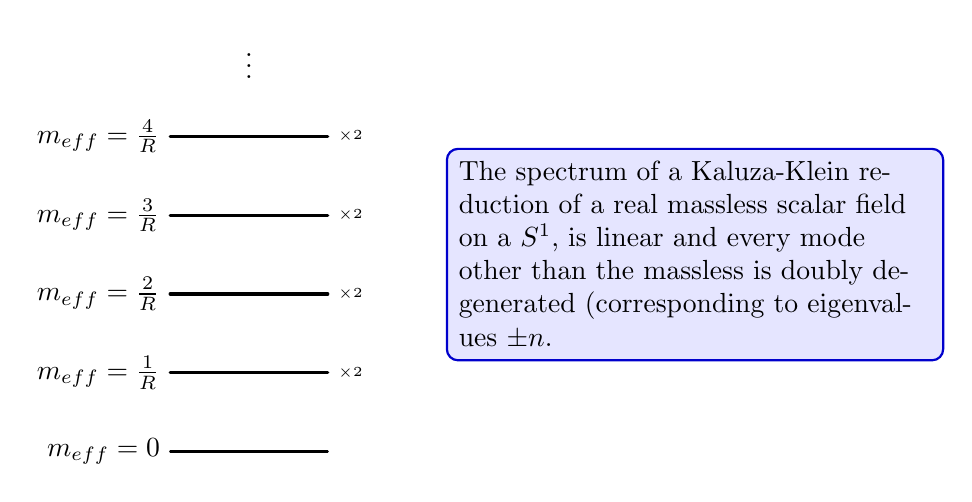
\begin{tikzpicture}[thick,line cap=round,
      % Styles
      axes/.style=,
      important line/.style={very thick},
      information text/.style={rounded corners,draw=blue!80!black,fill=blue!10,inner sep=1ex}]
    
    \draw (0,0) node[anchor=east] {$m_{\text{eff}} =0$} -- (2,0);
    \foreach \y in {1,2,...,4}
    \draw[important line] (0,\y) node[anchor=east] {$m_{\text{eff}} =\frac{\y}{R}$} -- (2,\y);
    \foreach \y in {1,2,...,4}
    \node[anchor=west] at (2,\y) {{\tiny $ \times 2$}};

    \node at (1,5) {$\vdots$};

    \draw[xshift=3.5cm,yshift=2.5cm]
    node[right,text width=6cm,information text]
    {The spectrum of a Kaluza-Klein reduction of a real massless scalar field on a $S^1$, is linear and every mode other than the massless is doubly degenerated (corresponding to eigenvalues $\pm n$.};
  \end{tikzpicture}
\end{center}

\subsection{Scalar Field Reduced on $S^2$}

One can follow the previous procedure to compute the \KK of a massless real scalar field on $S^2$. Thus, assuming that $M^{D+1}=M^D\times S^2$, the differential operator separates on,
\begin{align}
  \(\Box^{(D)}+\Lap\)\Phi =0.\label{KKs-eq:s2}
\end{align}
Then, the \KK ansatz is done as an expansion on eigenfunctions of the 2-dimensional Laplacian on spherical coordinates, i.e., spherical harmonics, as
\begin{align}
  \Phi(x,\xi) = \sum_{l,m} \phi_{l,m}(x)Y^{lm}(\xi),
\end{align}
where $Y^{lm}$ satisfy
\begin{align}
  \Lap Y^{lm} = -\frac{l(l+1)}{R^2} Y^{lm}.
\end{align}

Therefore, Eq. \eqref{KKs-eq:s2} yields
\begin{align}
  \[\Box^{(D)}-\frac{l(l+1)}{R^2}\]\phi_{l,m}(x) =0.\label{KK-eq-s2}
\end{align}
Eq. \eqref{KK-eq-s2} represents a \KK tower composed by: a single massless scalar field, corresponding to $l=0$; and $(2l+1)$-degenerated massive scalar fields with and effective mass
\begin{align}
  m_{\text{eff}} = \frac{\sqrt{l(l+1)}}{R}.
\end{align}

\begin{center}
  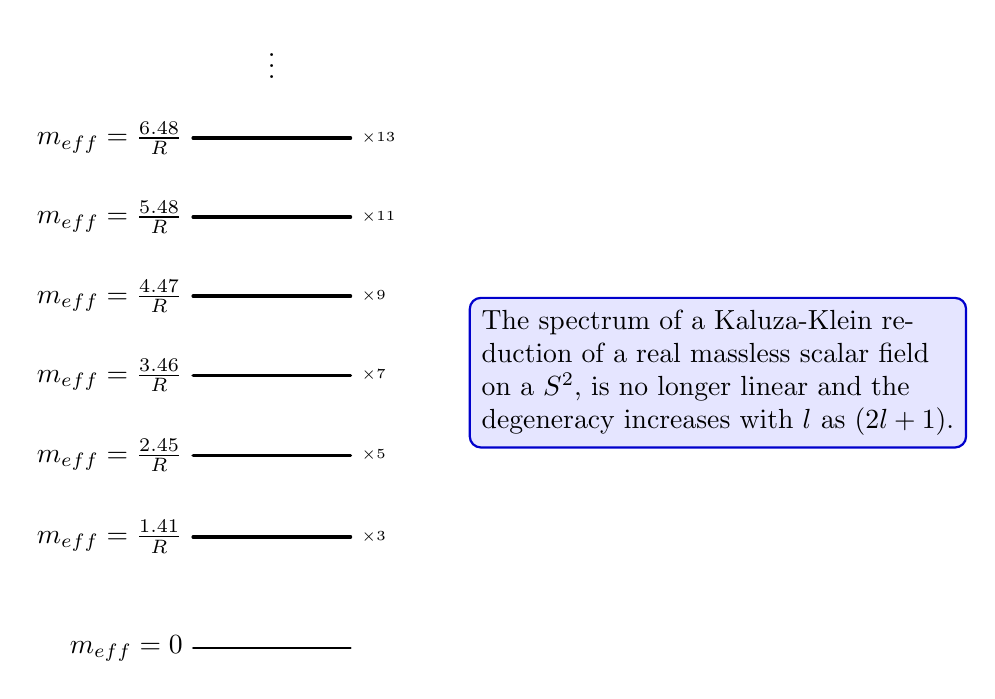
\begin{tikzpicture}[thick,line cap=round,
      % Styles
      axes/.style=,
      important line/.style={very thick},
      information text/.style={rounded corners,draw=blue!80!black,fill=blue!10,inner sep=1ex}]
    \pgfkeys{/pgf/number format/.cd,fixed,precision=2}

    \draw (0,0) node[anchor=east] {$m_{\text{eff}} =0$} -- (2,0);
    \foreach \y/\m in {1/3,2/5,3/7,4/9,5/11,6/13}
    {
      \draw[important line] (0,{sqrt(\y*\y + \y) }) node[anchor=east] {$m_{\text{eff}} =\frac{\pgfmathparse{sqrt(\y*\y + \y) }\pgfmathprintnumber{\pgfmathresult}}{R}$} -- (2,{sqrt(\y*\y + \y) }) node[anchor=west]  {{\tiny $ \times\m$}};
    }
    \node at (1,7.5) {$\vdots$};

    \draw[xshift=3.5cm,yshift=3.5cm]
    node[right,text width=6cm,information text]
    {The spectrum of a Kaluza-Klein reduction of a real massless scalar field on a $S^2$, is no longer linear and the degeneracy increases with $l$ as $(2l+1)$.};
  \end{tikzpicture}
\end{center}

\subsection{Scalar Field Reduced on $T^2$}

Once more, inspired in the previous procedure, and using the fact that $T^2=S^1\times S^1$, the differential operator separates on,
\begin{align}
  \(\Box^{(D)}+\pa{\xi_1}^2+\pa{\xi_2}^2\)\Phi =0,\label{KKs-eq:t2}
\end{align}
and the \KK ansatz is
\begin{align}
  \Phi(x,\xi) = \sum_{m,n} \phi_{m,n}(x) e^{\imath \(\frac{m}{R_1}\xi_1 + \frac{n}{R_2}\xi_2\)},\label{KK-scalar:t2}
\end{align}
where $R_1$ and $R_2$ are the radii of the torus.

Substituting the expansion \eqref{KK-scalar:t2} into \eqref{KKs-eq:t2}, yields
\begin{align}
  \[\Box^{(D)}-\(\frac{m}{R_1}\)^2-\(\frac{n}{R_2}\)^2\]\phi_{m,n}(x)=0\qquad \forall\; m,n\in \Z.\label{KK-eq-t2}
\end{align}

Eq. \eqref{KK-eq-t2} represents a tower of \KK modes which contains a massless singlet, and infinite massive modes whose degeneracy depend on the relation between the integers $m,n$ and the radii $R_1$ and $R_2$. The effective mass for the \KK modes is
\begin{align}
  m_{\text{eff}} =  \sqrt{\(\frac{m}{R_1}\)^2+\(\frac{n}{R_2}\)^2}.
\end{align}

\begin{center}
  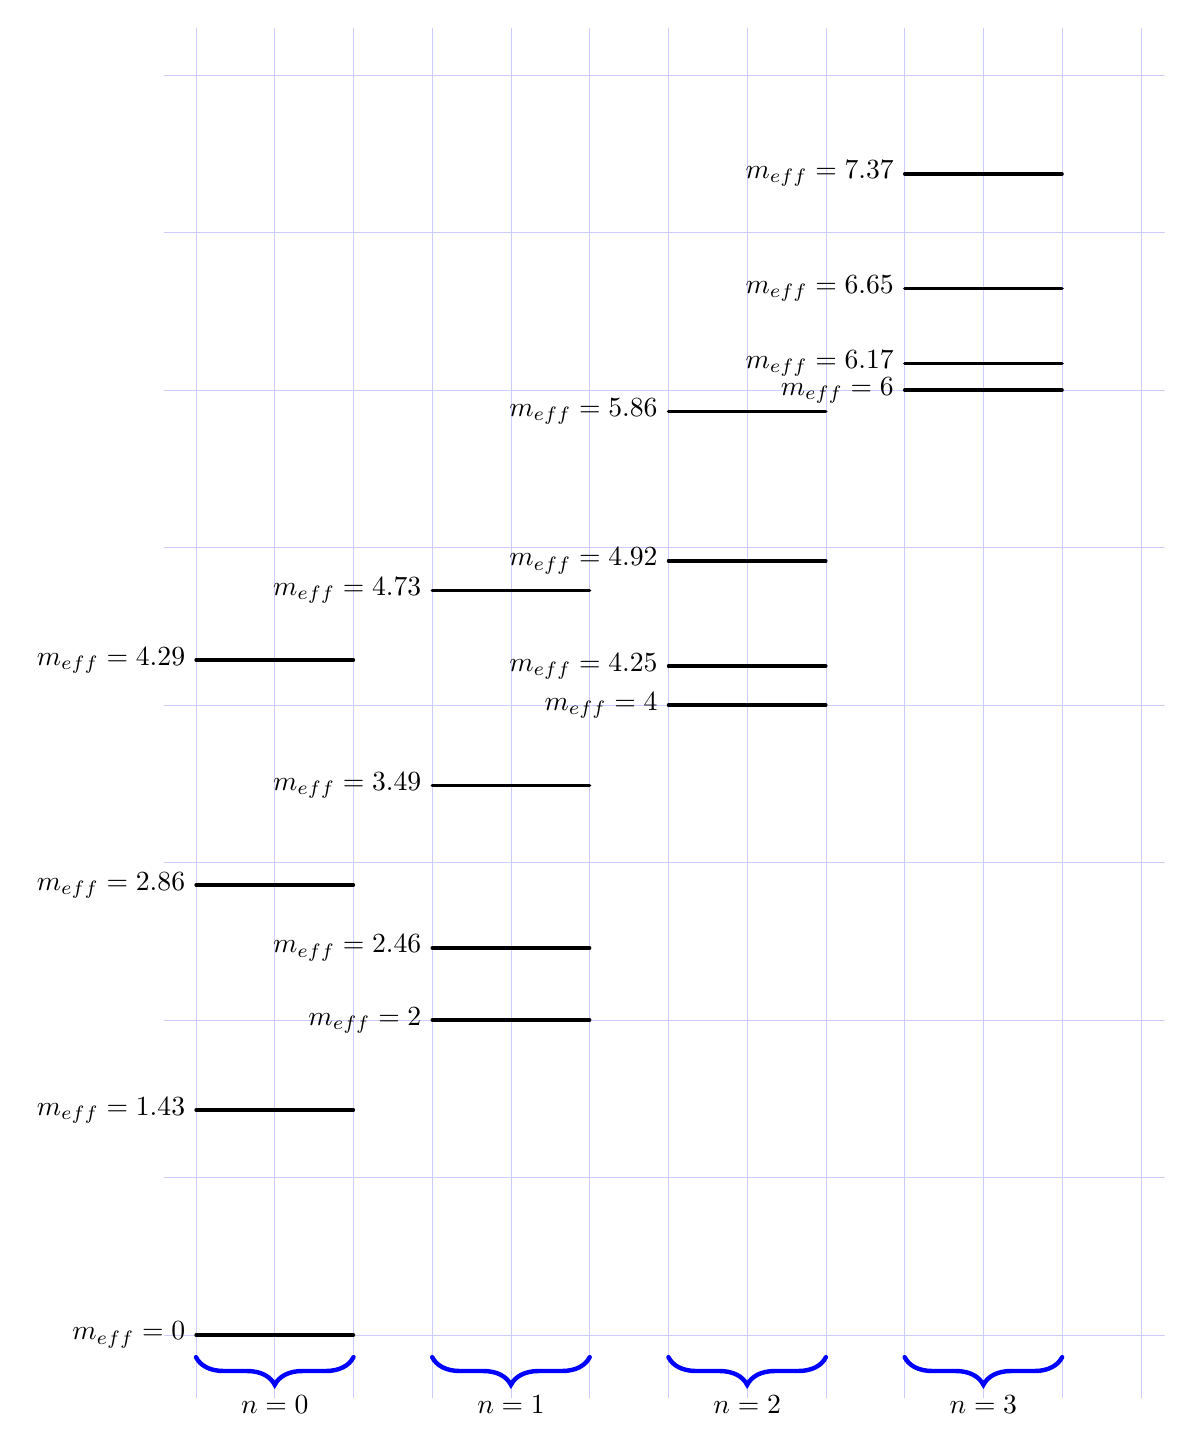
\begin{tikzpicture}[thick,line cap=round,yscale=2,
      % Styles
      axes/.style=,
      important line/.style={very thick},
      information text/.style={rounded corners,draw=blue!80!black,fill=blue!10,inner sep=1ex}]
    \pgfkeys{/pgf/number format/.cd,fixed,precision=2}

    \pgfmathsetmacro{\r}{.7}
    \pgfmathsetmacro{\R}{.5}
    
    \draw[help lines, color=blue!20,step=1cm] (-.4,-.4) grid (12.3,8.3);

    %\draw (0,0) node[anchor=east] {$m_{\text{eff}} =0$} -- (2,0);
    \foreach \n in {0,1,2,3}  {
      \foreach \m in {0,1,...,3} {
        \draw[important line,xshift=3*\n cm] (0,{sqrt((\m/\r)^2 + (\n/\R)^2)}) node[anchor=east] {$m_{\text{eff}} = \pgfmathparse{sqrt((\m/\r)^2 + (\n/\R)^2) }\pgfmathprintnumber{\pgfmathresult}$} -- (2,{sqrt((\m/\r)^2 + (\n/\R)^2)});
        }
      \draw [decorate,decoration={brace,amplitude=10pt,mirror},ultra thick,color=blue,yshift=-4pt,xshift=3*\n cm] (0,0) -- (2,0) node [black,midway,yshift=-0.6cm] { $n=\n$};
      }
    
    
  \end{tikzpicture}
\end{center}

\section{Kaluza-Klein Reduction on $S^1$}

\begin{equation}
  d\hat{s}^2 = e^{2\alpha\phi}ds^2 + e^{2\beta\phi}\left(d\xi + \Ag\right)^2,
\end{equation}

\begin{equation}
\VIF{a} = 
\begin{cases}
  \hvif{a} = e^{\alpha\phi} \vif{a}\\
  \hvif{D} = e^{\beta\phi}\left(\df\;\xi +\Ag \right)
\end{cases},
\end{equation}

From the first Maurer-Cartan equation,
\begin{equation}
  \df\VIF{a} + \SPIF{a}{b}\w\VIF{b} = {\bf{T}}^{\hat{a}} = 0,
\end{equation}
the spin connection can be calculated.
\begin{align}
  \df\hvif{D} =& e^{\beta\phi}\left[\beta\df\;\phi\w\left(\df\;\xi +\Ag \right) + \df\Ag\right]\nonumber\\
  =& e^{\beta\phi}\left[-\beta\left(\df\;\xi +\Ag \right)\w\df\;\phi + \df\Ag\right]\nonumber\\
  =& e^{\beta\phi}\left[-\beta\pa{a}\phi\left(\df\;\xi +\Ag \right)\w\vif{a} + \Fg\right]\nonumber\\
 =& -\beta e^{-\alpha\phi}\pa{a}\phi\;\hvif{D}\w\hvif{a} -\frac{1}{2}e^{(\beta-2\alpha)\phi}\F_{a b}\;\hvif{b}\w\hvif{a},
\end{align}
from where one gets,
\begin{align}
  \hspif{D}{a} = \beta e^{-\alpha\phi}\pa{a}\phi\hvif{D} + \frac{1}{2}e^{(\beta-2\alpha)\phi}\F_{a b}\hvif{b}.
\end{align}

On the other hand,
\begin{align}
  \hspif{a}{b}\w\hvif{b} = -\df\hvif{a} - \hspif{a}{D}\w\hvif{D}.
\end{align}
Since,
\begin{align}
  \df\hvif{a} 
  =& e^{\alpha\phi}\left[\alpha\df\;\phi\w\vif{a} +  \df\vif{a}\right]\nonumber\\
  =& e^{\alpha\phi}\left[-\alpha\vif{a}\w\df\;\phi -  \spif{a}{b}\w\vif{b}\right]\nonumber\\
  =& -\alpha e^{-\alpha\phi}\pa{b}\phi\;\hvif{a}\w\hvif{b} - \spif{a}{b}\w\hvif{b},
\end{align}
then,
\begin{align}
  \hspif{ab}{} =& \spif{ab}{} + \alpha e^{-\alpha\phi}\pau{b}\phi\hvif{a} - \frac{1}{2}e^{(\beta-2\alpha)\phi}\F^{a b}\hvif{D}\nonumber\\
  =& \spif{ab}{} + \alpha e^{-\alpha\phi}\left(\pau{b}\phi\hvif{a} - \partial^{a}\phi\hvif{b}\right) - \frac{1}{2}e^{(\beta-2\alpha)\phi}\F^{a b}\hvif{D}.
\end{align}

Now, the second Maurer-Cartan equation,
\begin{align}
  \df\SPIF{a}{b}+\SPIF{a}{c}\w\SPIF{c}{b}=\RIF{a}{b}.
\end{align}

\begin{align}
  \df\hspif{D a}{} 
  =& \beta\;\df\left( e^{-\alpha\phi}\pau{a}\phi\;\hvif{D}\right) + \frac{1}{2}\df\left(e^{(\beta-2\alpha)\phi}\F^a{}_{b}\;\hvif{b}\right)\nonumber\\
  =& \beta e^{-\alpha\phi}\;\left[-\alpha \pau{a}\phi\;\df\;\phi\w\hvif{D} +\pau{a}\df\;\phi\w\hvif{D} + \pau{a}\phi\;\df\hvif{D}\right]\notag\\
  & + \frac{1}{2}e^{(\beta-2\alpha)\phi}\left[(\beta-2\alpha)\F^a{}_{b}\;\df\;\phi\w\hvif{b} + \df \F^a{}_{b}\w\hvif{b} + \F^a{}_{b}\;\df\hvif{b}\right]\nonumber\\
  =& \beta e^{-\alpha\phi}\;\left[-\alpha \pau{a}\phi\pa{b}\phi\;\vif{b}\w\hvif{D} +\pau{a}\pa{b}\phi\;\vif{b}\w\hvif{D} + \pau{a}\phi\;\hspif{D}{b}\w\hvif{b}\right] \notag\\
  &+ \frac{1}{2}e^{(\beta-2\alpha)\phi}\left[(\beta-2\alpha)\F^a{}_b\pa{c}\phi\;\vif{c}\w\hvif{b} + \pa{c} \F^a{}_b\;\vif{c}\w\hvif{b} + \F^a{}_b\;\hspif{b}{\hat{c}}\w\VIF{c}\right]\nonumber\\
 =& \beta(\beta-\alpha)e^{-2\alpha\phi}\pau{a}\phi\pa{b}\phi\;\hvif{b}\w\hvif{D} + \beta e^{-2\alpha\phi}\pau{a}\pa{b}\phi\;\hvif{b}\w\hvif{D}  \notag\\
 &-\frac{\beta-\alpha}{2}e^{(\beta-3\alpha)\phi}\F^a{}_b\pa{c}\phi\;\hvif{b}\w\hvif{c} +\frac{\beta}{2}e^{(\beta-3\alpha)\phi}\pau{a}\phi \F_{bc}\;\hvif{b}\w\hvif{c}\nonumber\\
 & -\frac{1}{2}e^{(\beta-3\alpha)\phi}\pa{c} \F^a{}_b\;\hvif{b}\w\hvif{c} - \frac{1}{2}e^{(\beta-2\alpha)\phi}\F^a{}_b\; \spif{b}{c}\w\hvif{c},
\end{align}
and,
\begin{align}
  \hspif{D}{m}\w\hspif{m a}{} =& \left(\beta e^{-\alpha\phi}\pa{m}\phi\;\hvif{D} + \frac{1}{2}e^{(\beta-2\alpha)\phi}\F_{m b}\;\hvif{b}  \right)\w\notag\\
  &{}\;\left(\spif{m a}{} + \alpha e^{-\alpha\phi}\left(\pau{a}\phi\;\hvif{m} - \partial^{m}\phi\;\hvif{a}\right) - \frac{1}{2}e^{(\beta-2\alpha)\phi}\F^{m a}\;\hvif{D}  \right)\nonumber\\
 =& \beta e^{-\alpha\phi}\pa{m}\phi\;\hvif{D}\w\spif{m a}{} + \alpha\beta e^{-2\alpha\phi}\pa{m}\phi\;\hvif{D}\w\left(\pau{a}\phi\;\hvif{m} - \partial^{m}\phi\;\hvif{a}\right)\nonumber\\
 & + \frac{1}{2}e^{(\beta-2\alpha)\phi}\F_{m b}\;\hvif{b}\w\spif{m a}{} + \frac{\alpha}{2}e^{(\beta-3\alpha)\phi}\F_{m b}\;\hvif{b}\w\left(\pau{a}\phi\;\hvif{m} - \partial^{m}\phi\;\hvif{a}\right)\nonumber\\
 & -\frac{1}{4}e^{2(\beta-2\alpha)\phi}\F_{m n}\F^{m a}\;\hvif{n}\w\hvif{D}.
\end{align}
Therefore,
\begin{align}
  \hRif{D a}{} =& - \frac{1}{2}e^{(\beta-2\alpha)\phi}\(\F_{bc}\spif{ba}{} + \F^a{}_{b}\; \spif{b}{c}\)\w\hvif{c} + \beta e^{-\alpha\phi}\pa{m}\phi\;\spif{m a}{}\w\hvif{D} \notag\\
  & + \[\beta e^{-2\alpha\phi}\big((\beta-2\alpha)\pa{b}\phi\pau{a}\phi + \pa{b}\pau{a}\phi\big) -\frac{1}{4} e^{2(\beta-2\alpha)\phi}\F_{cb}\F^{ca} \]\hvif{b}\w\hvif{D}\notag\\
  & + \frac{e^{(\beta-3\alpha)\phi}}{2}\bigg[ (\beta-\alpha)\big(\pau{a}\phi\F_{mb} +\pa{m}\phi\F^a{}_b  \big) + \pa{m}\F^a{}_b \bigg] \hvif{m}\w\hvif{b} \notag\\
  & +\alpha\beta e^{-2\alpha\phi}\pa{m}\phi\partial^{m}\phi \;\hvif{a}\w\hvif{D} -\frac{\alpha}{2}e^{(\beta-3\alpha)\phi}\pau{b}\phi\F_{bc}\;\hvif{c}\w\hvif{a}
\end{align}

The second term,
\begin{align}
  \df\hspif{ab}{} =&\quad \df \spif{ab}{} + \df\[\alpha e^{-\alpha\phi}\(\pau{b}\phi\hvif{a}-\pau{a}\phi\hvif{b}\)\]-\frac{1}{2}\df\[e^{(\beta-2\alpha)\phi}\F^{ab}\hvif{D}\]\notag\\
  =&\quad \df \spif{ab}{} + \alpha^2 e^{-2\alpha\phi}\pa{c}\phi\(\pau{b}\phi\hvif{a}-\pau{a}\phi\hvif{b}\)\w\hvif{c}\notag\\
  &\quad -\alpha e^{-2\alpha\phi}\(\pa{c}\pau{b}\phi\hvif{a}-\pa{c}\pau{a}\phi\hvif{b}\)\w\hvif{c}  + \alpha e^{-\alpha\phi}\(\pau{b}\phi\df\hvif{a}-\pau{a}\phi\df\hvif{b}\)\notag\\
  &\quad-\frac{1}{2} e^{(\beta-3\alpha)\phi}\[(\beta-2\alpha)\pa{c}\phi \F^{ab} + \pa{c}\F^{ab}\]\hvif{c}\w\hvif{D}\notag\\
  &\quad  -\frac{1}{2}e^{(\beta-2\alpha)\phi}\F^{ab}\df\hvif{D}\notag\\
  =&\quad \df \spif{ab}{} -\alpha e^{-2\alpha\phi}\(\pa{c}\pau{b}\phi\hvif{a}-\pa{c}\pau{a}\phi\hvif{b}\)\w\hvif{c} \notag\\
  &\quad - \alpha e^{-\alpha\phi}\(\pau{b}\phi\spif{a}{m}-\pau{a}\phi\spif{b}{m}\)\w\hvif{m}-\frac{1}{4} e^{2(\beta-2\alpha)\phi}\F^{ab}\F_{mn}\hvif{m}\w\hvif{n}\\
  &\quad - \frac{1}{2} e^{(\beta-3\alpha)\phi}\[2(\beta-\alpha)\pa{c}\phi \F^{ab} + \pa{c}\F^{ab}\]\hvif{c}\w\hvif{D},\notag%\\
\end{align}
and 
\begin{align}
  \hspif{a}{D}\w\hspif{D b}{} =&\quad -\(  \beta e^{-\alpha\phi}\pau{a}\phi\hvif{D} + \frac{1}{2}e^{(\beta-2\alpha)\phi}\F^{a}{}_m\hvif{m} \)\w\( \beta e^{-\alpha\phi}\pau{b}\phi\hvif{D} + \frac{1}{2}e^{(\beta-2\alpha)\phi}\F^{b}{}_n\hvif{n} \)\notag\\
  =&\quad +\frac{\beta}{2}e^{(\beta-3\alpha)\phi}\(\pau{a}\phi \F^{b}{}_m -\pau{b}\phi\F^{a}{}_m\)\hvif{m}\w\hvif{D}%\notag\\
  %&\quad 
  -  \frac{1}{4}e^{2(\beta-2\alpha)\phi}\F^{a}{}_m \F^{b}{}_n\hvif{m}\w\hvif{n}
\end{align}
\begin{align}
  \hspif{a}{c}\w\hspif{c b}{}  =&\quad \spif{a}{c}\w\spif{c b}{} +\frac{1}{2}e^{(\beta-2\alpha)\phi}\(\F^{a}{}_c \spif{cb}{} -\F^{b}{}_c\spif{ca}{}\)\w\hvif{D}\notag\\
  &\quad +\alpha e^{-\alpha\phi}\( \pau{b}\phi\spif{a}{c}\w\hvif{c} -\pau{c}\phi\spif{a}{c}\w\hvif{b} + \pau{c}\phi\spif{b}{c}\w\hvif{a} - \pau{a}\phi\spif{b}{c}\w\hvif{c}  \) \notag\\
  &\quad +\alpha^2 e^{-2\alpha\phi}\( \pau{b}\phi\pa{c}\phi\hvif{a}\w\hvif{c} -\pau{a}\phi\pa{c}\phi\hvif{b}\w\hvif{c} - \pau{c}\phi\pa{c}\phi\hvif{a}\w\hvif{b}  \) \notag\\
  &\quad +\frac{\alpha}{2}e^{(\beta-3\alpha)\phi}\[\F^b{}_c\(\pau{c}\phi\hvif{a} - \pau{a}\phi\hvif{c}\)  + \F^a{}_c\(\pau{b}\phi\hvif{c} - \pau{c}\phi\hvif{b}\)   \]\w\hvif{D}.
\end{align}

Next, one can write the Lagrangian of the higher dimensional spacetime,
\begin{align}
  \Lag_{(D+1)} =& \frac{\epsilon_{\hat{a}_1\hat{a}_2\cdots\hat{a}_{D+1}}}{(D-1)!}\hRif{\hat{a}_1\hat{a}_2}{}\w\hvif{\hat{a}_3}\w\cdots\w\hvif{\hat{a}_{D+1}}\\
  =& \underbrace{2\frac{\epsilon_{D a_1 a_2\cdots a_{D}}}{(D-1)!}\hRif{D{a}_1}{}\w\hvif{{a}_2}\w\cdots\w\hvif{{a}_{D}}}_{\text{Term }I}\notag\\
  &+ \underbrace{\frac{\epsilon_{a_1 a_2\cdots a_{D}D}}{(D-2)!}\hRif{{a}_1{a}_2}{}\w\hvif{{a}_3}\w\cdots\w\hvif{{a}_{D}}\w\hvif{D}}_{\text{Term }II}.
\end{align}
Concentrate on the first term,
\begin{align}
  I =&\quad 2(-1)^D \frac{\epsilon_{a_1 a_2\cdots a_{D}}}{(D-1)!}\notag\\
  &\qquad\bigg\{\[\beta e^{-2\alpha\phi}\big((\beta-2\alpha)\pa{b}\phi\pau{a_1}\phi + \pa{b}\pau{a_1}\phi\big) -\frac{1}{4} e^{2(\beta-2\alpha)\phi}\F_{cb}\F^{ca_1} \]\hvif{b}\notag\\
  &\qquad + \beta e^{-\alpha\phi}\pa{m}\phi\;\spif{m a_1}{}+\alpha\beta e^{-2\alpha\phi}\pa{m}\phi\partial^{m}\phi \;\hvif{a}\bigg\}\w\hvif{D}\w\hvif{{a}_2}\w\cdots\w\hvif{{a}_{D}}\notag\\
  =&\quad -2\frac{\epsilon_{a_1 a_2\cdots a_{D}}}{(D-1)!}\notag\\
  &\qquad\bigg\{\[\beta e^{-2\alpha\phi}\big((\beta-2\alpha)\pa{b}\phi\pau{a_1}\phi + \pa{b}\pau{a_1}\phi\big) -\frac{1}{4} e^{2(\beta-2\alpha)\phi}\F_{cb}\F^{ca_1} \]\hvif{b}\notag\\
  &\qquad + \beta e^{-\alpha\phi}\pa{m}\phi\;\spif{m a_1}{}+\alpha\beta e^{-2\alpha\phi}\pa{m}\phi\partial^{m}\phi \;\hvif{a}\bigg\}\w\hvif{{a}_2}\w\cdots\w\hvif{{a}_{D}}\w\hvif{D}\notag\\
  =&\quad -2\frac{\epsilon_{a_1 a_2\cdots a_{D}}}{(D-1)!} e^{\((D-2)\alpha+\beta\)\phi}\notag\\
  &\qquad\bigg\{\[\beta \big((\beta-2\alpha)\pa{b}\phi\pau{a_1}\phi + \pa{b}\pau{a_1}\phi\big) -\frac{1}{4} e^{2(\beta-\alpha)\phi}\F_{cb}\F^{ca_1} \]\vif{b}\notag\\
  &\qquad + \beta \pa{m}\phi\;\(\spi{b}\)^{m a_1}\vif{b}+\alpha\beta \pa{m}\phi\partial^{m}\phi \;\vif{a_1}\bigg\}\w\vif{{a}_2}\w\cdots\w\vif{{a}_{D}}\w\df\;\xi\notag\\
  =&\quad -2 e^{\((D-2)\alpha+\beta\)\phi}\bigg\{\beta \big((\beta-2\alpha)\pa{b}\phi\pau{b}\phi + \pa{b}\pau{b}\phi\big)
    %% \notag\\
    %% &\qquad
-\frac{1}{4} e^{2(\beta-\alpha)\phi}\F_{cb}\F^{cb} \notag\\
  &\qquad\quad + \beta \pa{m}\phi\;\(\spi{b}\)^{m b} + D \alpha\beta \;\pa{m}\phi\partial^{m}\phi \bigg\}\de{V_D}\de{\xi}
\end{align}

\begin{align}
  II =&\quad \frac{\epsilon_{a_1 a_2\cdots a_{D}D}}{(D-2)!}\notag\\
  &\qquad \bigg\{\Rif{a_1a_2}{} -\alpha e^{-2\alpha\phi}\(\pa{c}\pau{a_2}\phi\hvif{a_1}-\pa{c}\pau{a_1}\phi\hvif{a_2}\)\w\hvif{c}\notag\\
  &\qquad -\frac{1}{4} e^{2(\beta-2\alpha)\phi}\(\F^{a_1a_2}\F_{mn}+\F^{a_1}{}_m \F^{a_2}{}_n\)\hvif{m}\w\hvif{n}\notag\\
  &\qquad +\alpha e^{-\alpha\phi}\( \pau{a_2}\phi\spif{a_1}{c}\w\hvif{c} -\pau{c}\phi\spif{a_1}{c}\w\hvif{a_2} + \pau{c}\phi\spif{a_2}{c}\w\hvif{a_1} - \pau{a_1}\phi\spif{a_2}{c}\w\hvif{c}  \) \notag\\
  &\qquad +\alpha^2 e^{-2\alpha\phi}\( \pau{a_2}\phi\pa{c}\phi\hvif{a_1}\w\hvif{c} -\pau{a_1}\phi\pa{c}\phi\hvif{a_2}\w\hvif{c} - \pau{c}\phi\pa{c}\phi\hvif{a_1}\w\hvif{a_2}  \) \notag\\
  &\qquad - \alpha e^{-\alpha\phi}\(\pau{a_2}\phi\spif{a_1}{m}-\pau{a_1}\phi\spif{a_2}{m}\)\w\hvif{m}\bigg\}\w\hvif{{a}_3}\w\cdots\w\hvif{{a}_{D}}\w\hvif{D}\notag\\
  =&\quad \frac{\epsilon_{a_1 a_2\cdots a_{D}}}{(D-2)!}e^{\((D-2)\alpha+\beta\)\phi}\notag\\
  &\qquad \bigg\{\Rif{a_1a_2}{} -\alpha \(\pa{c}\pau{a_2}\phi\vif{a_1}-\pa{c}\pau{a_1}\phi\vif{a_2}\)\w\vif{c}\notag\\
  &\qquad -\frac{1}{4} e^{2(\beta-\alpha)\phi}\(\F^{a_1a_2}\F_{mn}+\F^{a_1}{}_m \F^{a_2}{}_n\)\vif{m}\w\vif{n}\notag\\
  &\qquad +\alpha \( \pau{a_2}\phi\spif{a_1}{n}\w\vif{n} -\pau{c}\phi\spif{a_1}{c}\w\vif{a_2} + \pau{c}\phi\spif{a_2}{c}\w\vif{a_1} - \pau{a_1}\phi\spif{a_2}{n}\w\vif{n}  \) \notag\\
  &\qquad +\alpha^2 \( \pau{a_2}\phi\pa{c}\phi\vif{a_1}\w\vif{c} -\pau{a_1}\phi\pa{c}\phi\vif{a_2}\w\vif{c} - \pau{c}\phi\pa{c}\phi\vif{a_1}\w\vif{a_2}  \) \notag\\
  &\qquad - \alpha \(\pau{a_2}\phi\spif{a_1}{n}-\pau{a_1}\phi\spif{a_2}{n}\)\w\vif{n}\bigg\}\w\vif{{a}_3}\w\cdots\w\vif{{a}_{D}}\w\df\;\xi\notag\\
  =&\quad \frac{\epsilon_{a_1 a_2\cdots a_{D}}}{(D-2)!}e^{\((D-2)\alpha+\beta\)\phi} \notag\\
  &\qquad \bigg\{\Rif{a_1a_2}{}  - \alpha^2 \pau{c}\phi\pa{c}\phi\vif{a_1}\w\vif{a_2} \notag\\
  &\qquad  -\frac{1}{4} e^{2(\beta-\alpha)\phi}\(\F^{a_1a_2}\F_{mn}+\F^{a_1}{}_m \F^{a_2}{}_n\)\vif{m}\w\vif{n}\notag\\
  &\qquad +\alpha \[\alpha \pau{a_2}\phi\pa{c}\phi - \pa{c}\pau{a_2}\phi - \pau{m}\phi\(\spi{c}\)^{a_2}{}_{m}  \]\vif{a_1}\w\vif{c} \notag\\
  &\qquad -\alpha \[\alpha \pau{a_1}\phi\pa{c}\phi - \pa{c}\pau{a_1}\phi - \pau{m}\phi\(\spi{c}\)^{a_1}{}_{m}  \]\vif{a_2}\w\vif{c} \bigg\}\w\vif{{a}_3}\w\cdots\w\vif{{a}_{D}}\w\df\;\xi\notag\\
  =&\quad e^{\((D-2)\alpha+\beta\)\phi}\de{V_D}\de{\xi}\bigg\{\Ri - D(D-1)\alpha^2 \pau{c}\phi\pa{c}\phi - \frac{1}{4} e^{2(\beta-\alpha)\phi}\F_{mn}\F^{mn}\notag\\
  &\qquad + 2(D-1)\alpha \big[\alpha \pau{c}\phi\pa{c}\phi - \pa{c}\pau{c}\phi - \pau{m}\phi\(\spi{c}\)^{c}{}_{m}  \big]\bigg\}
\end{align}

Therefore,
\begin{align}
  \Lag_{(D+1)} =&\quad  e^{\((D-2)\alpha+\beta\)\phi}\de{V_D}\de{\xi}\bigg\{\Ri - D(D-1)\alpha^2 \pau{c}\phi\pa{c}\phi - \frac{1}{4} e^{2(\beta-\alpha)\phi}\F_{mn}\F^{mn}\notag\\
  &\qquad + 2(D-1)\alpha \big[\alpha \pau{c}\phi\pa{c}\phi - \pa{c}\pau{c}\phi - \pau{m}\phi\(\spi{c}\)^{c}{}_{m}  \big]\notag\\
  &\qquad -2\beta \big((\beta-2\alpha)\pa{b}\phi\pau{b}\phi + \pa{b}\pau{b}\phi\big) +\frac{1}{2} e^{2(\beta-\alpha)\phi}\F_{cb}\F^{cb} \notag\\
  &\qquad -2 \beta \pa{m}\phi\;\(\spi{b}\)^{m b} -2 D \alpha\beta \;\pa{m}\phi\partial^{m}\phi \bigg\}\notag\\
  =&\quad  e^{\((D-2)\alpha+\beta\)\phi}\de{V_D}\de{\xi}\bigg\{\Ri - \[(D-1)(D-2)\alpha^2 +2\beta(\beta-2\alpha) + 2D\alpha\beta\]\pau{c}\phi\pa{c}\phi\notag\\
  &\qquad + \frac{1}{4} e^{2(\beta-\alpha)\phi}\F_{mn}\F^{mn} - 2\[(D-1)\alpha +\beta\]\Box\phi - 2\[(D-1)\alpha -\beta\]\pa{m}\phi\(\spi{c}\)^{cm}\bigg\}
\end{align}

One can choose $\beta=-(D-2)\alpha$, so that the result on the compactification would give $D$-dimensional gravity on the ``Einstein'' frame, then
\begin{align}
  \Lag_{(D+1)} =&\quad  \de{V_D}\de{\xi}\bigg\{\Ri - (D-1)(D-2)\alpha^2\pau{c}\phi\pa{c}\phi\notag\\
  &\qquad + \frac{1}{4} e^{-2(D-1)\alpha\phi}\F_{mn}\F^{mn} \bigg\},%- 2\[(D-1)\alpha +\beta\]\Box\phi - 2\[(D-1)\alpha -\beta\]\pa{m}\phi\(\spi{c}\)^{cm}\bigg\}
\end{align}
where the other terms were dropped because are a boundary term. Additionally, in order to get the usual kinetic term for the scalar field, i.e., 
\begin{align}
  \alpha^2 = \frac{1}{2}\frac{1}{(D-1)(D-2)},
\end{align}
finally
\begin{align}
  \Lag_{(D+1)} =\;  \de{V_D}\de{\xi}\bigg\{\Ri - \frac{1}{2}\pau{c}\phi\pa{c}\phi + \frac{1}{4} e^{-2(D-1)\alpha\phi}\F_{mn}\F^{mn} \bigg\}.
\end{align}

\chapter{More Advanced \KK Reduction}

In the previous chapter, it was seen that the \KK reduction of a scalar field on a total spacetime, which is a direct product of a $D$-dimensional spacetime and a compact manifold, is done with ease, but the moral of the procedure is that the effective mass is inversely proportional to the typical length, {\it a.k.a.} radius, of the compact manifold.

Therefore, if there is a phenomenological argument to assume that the compact manifold has a typical radius $R\lll \SI{e-2}{\TeV}$, then only the massless modes of the effective theory are worth tho be analysed. Thus, it is necessary to learn how to count the number of massless fields on the lower dimensional theory. The task is achieved by using topological information of the compact manifold.

\section{Massless Fields and Harmonic Forms}

It was shown in the three examples in Sec.~\ref{sec:KKs:s1}, Sec.~\ref{sec:KKs:s2} and Sec.~\ref{sec:KKs:t2}, when the \KK reduction is done on a compact manifold, $\mathcal{K}$, the massless scalar fields come from the number of nonequivalent harmonic forms on $\mathcal{K}$. This number is independent of the geometry of $\mathcal{K}$, which can be heuristically argued from the fact that is independent or $R$, but is a topological quantity, i.e., a topological invariant.

In a previous chapter, the de Rham cohomology group\index{Cohomology group!de Rham} was defined as
\begin{equation}
  H^p(M) \equiv \frac{ \Ker \( \df : C^\infty \( \Lambda^{p}(M) \) \to C^\infty \( \Lambda^{p+1}(M) \) \) }{ \Im \( \df : C^\infty \( \Lambda^{p-1}(M) \) \to C^\infty \( \Lambda^{p}(M) \) \) },
\end{equation}
therefore, the number of nonequivalent harmonic $p$-forms equals the dimension of the $p$-th de Rham cohomology group, which is commonly known as the $p$-th \idx{Betti number}, $b^p(M)$.

From the previous paragraph, the number of massless scalar fields in the lower dimensional effective theory is $b^0(M)$, while the number of massless 1-forms is $b^1(M)$, and so on! 
Nonetheless, the counting is not necessarily right, since the dimensional reduction of $p$-forms on a compact $n$-dimensional manifold yields to all kind of forms from $(p-n)$ to $p$ order.

In the next sections a heuristic way to compute Betti numbers of simple manifold is shown, and the dimensional reduction of a rich theory is considered.


\section{Cohomology and Homology}

The cohomology groups are not intuitive to calculate. However, de Rham showed that there is a duality between the cohomology group and the homology group.


\begin{Thm}
  \label{thm:dR}
  If $M$ is a compact manifold, $H^r (M)$ and
  $H_r (M)$ are finite dimensional. Moreover the exists a map
  \begin{equation}
    \Lambda    : H^r (M) \times H_r (M) \to \R,
  \end{equation}
  which is bilinear and non-degenerate. Thus, $H^ r (M)$ is the dual vector space of $H_r (M)$.
\end{Thm}

From Thm.~\ref{thm:dR}, it follows that $b^r(M) = \dim( H^r(M) ) = \dim( H_r(M) )$, and the later is nothing but the number of nonequivalent, un-shrinkable, $r$-cycles (modulus $r$-boundaries) defined on $M$.  These $r$-cycles can be count via the homotopy group, $\pi_r(M): S^r \to M$.


%% \begin{center}
%%   \begin{tikzpicture}
%%     \begin{axis}[
%%           hide axis,
%%           view={40}{40}
%%       ]
      
%%       \addplot3 [
%%         surf, shader=faceted interp,
%%         point meta=x,
%%         colormap/greenyellow,
%%         samples=20,
%%         samples y=40,
%%         %z buffer=sort,
%%         domain=0:180,
%%         y domain=0:360
%%       ] (
%%                 {sin(x)*cos(y)},
%%                 {sin(x)*sin(y)},
%%                 {cos(x)}
%%       );
      
%%     \end{axis}
%%   \end{tikzpicture}
%% \end{center}

Since the formal theory of this topological invariant is far from the scope of this manuscript, only examples are given in which the $r$-cycles are counted, and finally the {K\"unneth formula} for calculating the Betti numbers of Cartesian products of manifolds is stated.

\subsection{Betti Numbers Though Examples}

Concentrate in the $\pi_0(M)$, for an arbitrary manifold $M$. Since $S^0$ is a point, $b_0(M)$ counts the number of nonequivalent points on $M$, i.e., the number of connected components. Thus,
\begin{align}
  b_0(\R^n) = b_0(S^n) &= b_0(T^n) = 1, & & \\
  b_0(O(N))            &= 2            & &\text{for }N>1,
\end{align}
in the last line, $O(N)$ is the $N$-th orthogonal group, and the result is 2 because $O(N)$ has two disconnected components: transformations with $\det(M) = 1$ and transformations with $\det(M) = -1$.

One car restate the geometrical meaning of the zeroth Betti number as follows:
\begin{itemize}
\item Imagine a two-dimensional plane.
\item In order to cut it in two parts, one should take out a one-dimensional sub-manifold which can be closed, essentially $S^1$,  or open $\R^1$.
\item This taking out is nothing but a (2-1)-dimensional ``hole'' on $\R^2$. Or in other words, this transformed the connected manifold into two disconnected ones.
\end{itemize}
Therefore, in general the zeroth Betti number counts how many $(D-1)$-dimensional holes  are in a given manifold.

In  the same spirit than before, one can consider $\pi_1(M)$, the set of maps from $S^1 \to M$, and count the number of (independent) non-contractible ones. Below,%In Fig. \ref{fig:shrink}, 
the contraction  of a (blue) $S^1$ path to a (red) point is shown.
\begin{center}
  \begin{center}
    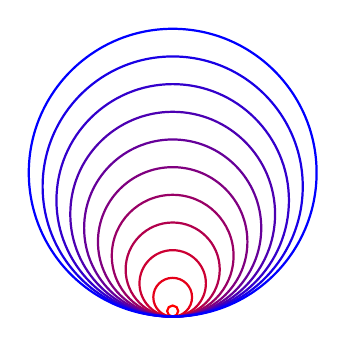
\begin{tikzpicture}[thick]
      \foreach \r in {0,10,...,100}
      \draw[color=blue!\r!red] (0,0) arc  (-90:270:2+.5*\r pt);
    \end{tikzpicture}
  \end{center}
\end{center}

If $M$ is a connected two-dimensional manifold, every circumference should be shrinkable, unless one of the points inside the circumference does not belong to $M$. Therefore,
\begin{gather}
  b_0(\R^n) = b_0(S^n) = 0, \\
  b_0\( \R^2 - \{0\} \) = 1.
\end{gather}
Moreover, if one ``puncture'' the two-dimensional plane $n$ times, then \mbox{$b_0\( \R^2 - n \{0\} \) = n$.}
\begin{center}
  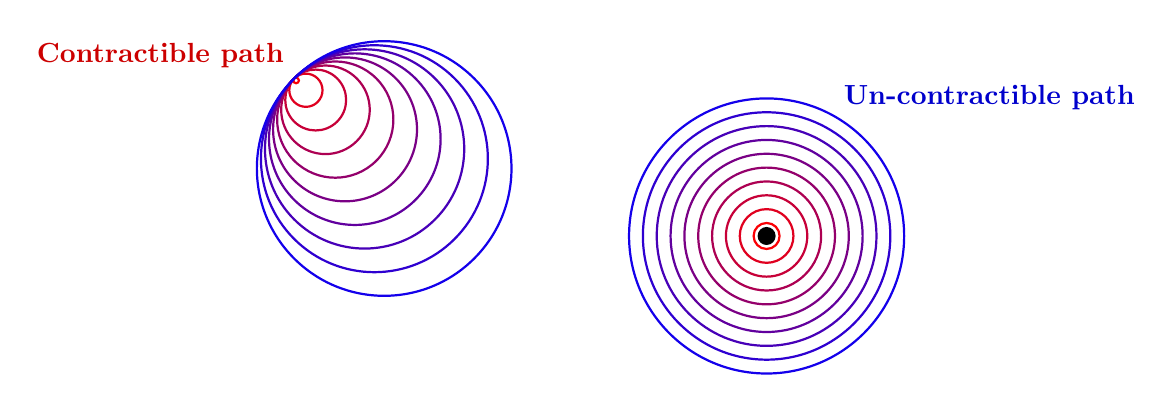
\begin{tikzpicture}[thick]
    \coordinate (P) at (8,2);
    \coordinate (O) at (2,4);
    %\draw[help lines, color=blue!20,step=1cm] (-.4,-.4) grid (12.3,8.3);
    \draw[fill=black] (P) circle (.1cm);
    \foreach \r in {2,12,...,92} {
      \draw[color=blue!\r!red] (O) arc  (-225:135:.5*\r pt);
      \draw[color=blue!\r!red] (P) circle (.5*\r pt+.13cm);}

    \node[anchor=south east] at (O) {\bf{\color{red!80!black}Contractible path}};
    \draw (60:1.7cm) ++(P) node[anchor=south west]   {\bf{\color{blue!80!black} Un-contractible path}};
  \end{tikzpicture}
\end{center}
Once more, a puncture on $\R^2$ is a $(D-2)$-dimensional hole. In fact, the first Betti number counts how many (independent) $(D-2)$-dimensional holes are in a given manifold.

The previous analysis can be carry on and on, and one reach the conclusion that the $n$-th Betti number counts how many independent $(D-n-1)$-dimensional holes are in a $D$-dimensional manifold $M$.



\section{K\"unneth formula}

When a manifold, $M$ is a Cartesian product of other manifolds, say $M_1$ and $M_2$, the topology is determined by the topology of the later. Therefore, their Betti numbers are related. The \idx{K\"unneth formula} shows that relation,
\begin{equation}
  b^n\(M=M_1\times M_2\) = \sum_{p+q=n} b^p\(M_1\)\cdot b^q\(M_2\).
  \label{KunnethForm}
\end{equation}

\begin{WEbox}[frametitle={Betti numbers of a torus ($T^n$)},
  frametitlerule=true,
  frametitlealignment=\centering,
  frametitleaboveskip=10pt,]
  Given the Betti numbers of the 1-sphere, $S^1$,
  \begin{equation}
    \begin{split}      
      b^0(S^1) &= 1, \notag \\
      b^1(S^1) &= 1,
    \end{split}
  \end{equation}
  one can calculate the Betti numbers of $T^n$, since $T^n = \times ^n S^1$.

  Using Eq.~\eqref{KunnethForm}, it follows that,
  \begin{equation}
    b^p(T^n) = \binom{n}{p} = \frac{n!}{p!(n-p)!}.
  \end{equation}
\end{WEbox}


\section{Kaluza-Klein spectrum of \M-theory}

The low energy limit of $\M$-theory is $D = 11$ supergravity, when  the spacetime is smooth and large compared with the $11$-dimensional Planck length. So, one can obtain the effective low energy description by consider Kaluza-Klein analysis~\cite{Papadopoulos:1995da,Acharya:2004qe}. 

Basically, one will consider the $11$-dimensional background $M^{10,1}$ as a reducible manifolds, $$M^{10,1} = M^{3,1} \times \mathcal{K},$$ where $M^{3,1}$ is a maximally symmetric spacetime and $\mathcal{K}$ is a compact $7$-dimensional manifold with holonomy group $G_2$.

The only bosonic fields in $D = 11$ supergravity are the metric $g$ and the $3$-form $C$. 

\subsection{Expansion of the $C$-form}

It is  considered that all vacuum expectation value for  the fields vanish, except the one of the metric. Then, considering fluctuations around the vacuum solution, it follows that
\begin{equation}
  C(x,y) = \delta C(x,y).
\end{equation}
Therefore, the equation of motion for $C$, 
\begin{equation}
  \ded G + \frac{1}{2} G \we G = 0,
  \label{eq:C}
\end{equation}
where $G = \ded C$, can be written to first order in $\delta C$ as
\begin{equation}
  \ded G = 0.
\end{equation}
As in Maxwell theory, one should impose the gauge condition $\ded C = 0$. Since $\La = \acomm{\dif}{\ded}$, finally the equation of motion is
\begin{equation}
  \La[11] C = 0.
\end{equation}

Now, splitting $\La[11] = \La[4] + \La[7]$, one notes that for the effective four-dimensional theory, the eigenvalues of $\La[7]$ are like  mass term. Therefore, one proceeds  expanding $C$ in term of the eigen-forms of $\mathcal{K}$.

One of the  assumptions of Kaluza-Klein approach is that %as one wants to consider extra dimensions with small radii
the radii of the extra dimensions is small. Then, the only interesting modes in the low energy four-dimensional theory are  massless states. This is because after compactifying the effective four-dimensional mass depends on radii as $m \sim \frac{1}{R}$, so if $R$ is ``really'' small, roughly speaking if it is of Planck length scale, which is $M_{\text{P}} \sim \SI{e-33}{\cm}$, the massive states are too heavy and they will not be considered in the low energy limit.

This allows  to consider the relevant expansion of $C$ just in terms of the harmonic forms on $\mathcal{K}$, as 
\begin{equation}
  C = \phi_I(x) \omega^I(y) + A_\alpha(x) \we \beta^\alpha(y) + \text{ (massive terms)},
\end{equation}
where $\omega^I$ are basis of the harmonic $3$-forms on $\mathcal{K}$, and $\beta^\alpha$ are basis of the harmonic $2$-forms on $\mathcal{K}$, so $I = 1, \cdots, b_3(\mathcal{K})$ and $\alpha = 1, \cdots, b_2(\mathcal{K})$, $x$ are coordinates along $M^4$ and $y$ are coordinates along $\mathcal{K}$. Since $C$ is odd under parity, $\phi_I$ describe $b_3(\mathcal{K})$ pseudo-scalars. On the other hand, $A_\alpha$ are  1-forms in Minkowski space, so, they are Abelian gauge fields in four-dimensions.

%% \chapter{Phi to the Fourth Theory}

\section{Leading order calculation of $Z[J]$}

\begin{align}
  Z_0[J] &= e^{-\frac{1}{2}\int \dn{4}{x}\dn{4}{x'}J(x)\Delta(x-x')J(x')} \notag\\
  &= e^{-\frac{1}{2}\vev{J\Delta J}},
\end{align}
and
\begin{align}
  Z[J] &= \No\[1+\(-\imath\frac{\lambda}{4!}\)\int \dn{4}{z}\(\frac{1}{\imath}\frac{\delta}{\delta J(z)}\)^4\]Z_0[J] \notag\\
  &= \No\[1 - \imath\frac{\lambda}{4!}\int \dn{4}{z}\(\frac{\delta}{\delta J_z}\)^4\]Z_0[J].
\end{align}
Then, the derivatives acting on $Z_0[J]$ yield,
\begin{align}
  \frac{\delta}{\delta J_z}Z_0[J] &= -\vev{\Delta J}_z Z_0[J],\\
  \frac{\delta^2}{\delta J_z^2}Z_0[J] &= \[- \Delta_{zz} + \vev{\Delta J}_z^2 \] Z_0[J],\\
  \frac{\delta^3}{\delta J_z^3}Z_0[J] &= \[ 3 \Delta_{zz}\vev{\Delta J}_z - \vev{\Delta J}_z^3 \] Z_0[J],\\
  \frac{\delta^4}{\delta J_z^4}Z_0[J] &= \[ 3 \Delta_{zz}{}^2 - 6 \Delta_{zz}\vev{\Delta J}_z^2 + \vev{\Delta J}_z^4 \] Z_0[J].
\end{align}
Therefore,
\begin{align}
  Z[J] &= \No\Bigg[Z_0[J] -\frac{\imath\lambda}{8}\int\dn{4}{z}\Delta_{zz}{}^2Z_0[J] + \frac{\imath\lambda}{4}\int\dn{4}{z}\Delta_{zz}\vev{\Delta J}_z^2Z_0[J]\notag\\
  &\qquad - \frac{\imath\lambda}{24}\int\dn{4}{z}\vev{\Delta J}_z^4 Z_0[J]\Bigg].\label{GenFun:firstorder}
\end{align}
These expression can be represented graphically, by using Feynman's diagrams, as follows
\begin{align}
  Z[J] = \No\[ 1
  - \frac{\imath\lambda}{8}\;
  
\begin{tikzpicture}[thick] %,baseline=(current bounding box)]
    \draw (2mm,0) circle (2mm);
    \draw (-2mm,0) circle (2mm);
  \end{tikzpicture}
  + \frac{\imath\lambda}{4}\;
  
\begin{tikzpicture}[thick]%,baseline=(current bounding box)]
    \draw plot[polar comb,mark=*] coordinates { (0:3mm) (180:3mm) };
    \draw (0,2mm) circle (2mm);
  \end{tikzpicture}
  - \frac{\imath\lambda}{24}\;
  
\begin{tikzpicture}[thick] %,baseline=(current bounding box)]
    \draw plot[polar comb,mark=*] coordinates { (45:3mm) (135:3mm) (-135:3mm) (-45:3mm) };    
  \end{tikzpicture}
  \] Z_0[J].
\end{align}

In order to find the normalisation factor, $\No$, one ask for
\begin{align}
  Z[J=0]=1,
\end{align}
then,
\begin{align}
  \No = \frac{1}{1 - \frac{\imath\lambda}{8}\int\dn{4}{z}\Delta_{zz}{}^2} \simeq 1 + \frac{\imath\lambda}{8}\int\dn{4}{z}\Delta_{zz}{}^2+\Or(\lambda^2),
\end{align}
which can be represented graphically by
\begin{align}
  \No = \frac{1}{1 - \frac{\imath\lambda}{8}\;
  
\begin{tikzpicture}[thick] %,baseline=(current bounding box.center)]
    \draw (2mm,0) circle (2mm);
    \draw (-2mm,0) circle (2mm);
  \end{tikzpicture}
  }
  = 1 + \frac{\imath\lambda}{8}\;
  
\begin{tikzpicture}[thick] %,baseline=(current bounding box.center)]
    \draw (2mm,0) circle (2mm);
    \draw (-2mm,0) circle (2mm);
  \end{tikzpicture}
  +\Or(\lambda^2).
\end{align}
Note that the normalisation factor is composed by ``vacuum bubbles'', and order by order this cancel the ``vacuum bubbles'' contribution to the calculation of the generating functional,
\begin{align}
  Z[J] &= \frac{1}{1 - \frac{\imath\lambda}{8}\;
  \begin{tikzpicture}[thick,baseline=-\the\dimexpr\fontdimen22\textfont2\relax] %,baseline=(current bounding box.center)]
    \draw (2mm,0) circle (2mm);
    \draw (-2mm,0) circle (2mm);
  \end{tikzpicture}
  }\[ 1
  - \frac{\imath\lambda}{8}\;
  \begin{tikzpicture}[thick,baseline=-\the\dimexpr\fontdimen22\textfont2\relax] %,baseline=(current bounding box)]
    \draw (2mm,0) circle (2mm);
    \draw (-2mm,0) circle (2mm);
  \end{tikzpicture}
  + \frac{\imath\lambda}{4}\;
  \begin{tikzpicture}[thick,baseline=-\the\dimexpr\fontdimen22\textfont2\relax]%,baseline=(current bounding box)]
    \draw plot[polar comb,mark=*] coordinates { (0:3mm) (180:3mm) };
    \draw (0,2mm) circle (2mm);
  \end{tikzpicture}
  - \frac{\imath\lambda}{24}\;
  \begin{tikzpicture}[thick,baseline=-\the\dimexpr\fontdimen22\textfont2\relax] %,baseline=(current bounding box)]
    \draw plot[polar comb,mark=*] coordinates { (45:3mm) (135:3mm) (-135:3mm) (-45:3mm) };    
  \end{tikzpicture}
  \] Z_0[J] \notag\\
  &= \[ 1
  + \frac{\imath\lambda}{4}\;
  \begin{tikzpicture}[thick,baseline=-\the\dimexpr\fontdimen22\textfont2\relax]%%,baseline=(current bounding box)]
    \draw plot[polar comb,mark=*] coordinates { (0:3mm) (180:3mm) };
    \draw (0,2mm) circle (2mm);
  \end{tikzpicture}
  - \frac{\imath\lambda}{24}\;
  \begin{tikzpicture}[thick,baseline=-\the\dimexpr\fontdimen22\textfont2\relax] %,baseline=(current bounding box)]
    \draw plot[polar comb,mark=*] coordinates { (45:3mm) (135:3mm) (-135:3mm) (-45:3mm) };    
  \end{tikzpicture}
  \] Z_0[J] \label{GenFun:FOgraph} \\
  &= \Bigg[1  + \frac{\imath\lambda}{4}\int\dn{4}{z}\Delta_{zz}\vev{\Delta J}_z^2 - \frac{\imath\lambda}{24}\int\dn{4}{z}\vev{\Delta J}_z^4\Bigg] Z_0[J].\label{GenFun:FO}
\end{align}

\section{Two-point Green's Function to First Order}

From the generating function, $Z[J]$, the $n$-point Green's function can be obtained through the relation
\begin{align}
  G^{(n)}(x_1,\cdots,x_n) = \left.\frac{1}{\imath^n}\frac{\delta^n Z[J]}{\delta J_1\cdots \delta J_n}\right|_{J=0}.
\end{align}

Therefore, from Eq.~\eqref{GenFun:FO} one obtains
\begin{align}
  G^{(2)}(x_1,x_2) &= -\left.\frac{\delta^2}{\delta J_1 \delta J_2}\[ 1 + \frac{\imath\lambda}{4}\int\dn{4}{z}\Delta_{zz}\vev{\Delta J}_z^2 - \frac{\imath\lambda}{24}\int\dn{4}{z}\vev{\Delta J}_z^4\] Z_0[J]\right|_{J=0} \notag\\
  &= -\[ -\Delta_{12} + \frac{\imath\lambda}{2}\int\dn{4}{z}\Delta_{zz}{\Delta }_{z1}{\Delta }_{z2}\] \notag\\
  &= 
  \begin{tikzpicture}[thick,baseline=-\the\dimexpr\fontdimen22\textfont2\relax] %,baseline=(current bounding box.center),scale=2]
    \draw (-3mm,0)   -- (3mm,0);
  \end{tikzpicture}
  - \frac{\imath\lambda}{2}\;
  \begin{tikzpicture}[thick,scale=2,baseline=-\the\dimexpr\fontdimen22\textfont2\relax] %]
    \draw (-3mm,0)  -- (3mm,0);
    \draw (0,2mm) circle (2mm);
  \end{tikzpicture}
\end{align}

\section{Four-point Green's Function to First Order}

From Eq.~\eqref{GenFun:FO}, and
\begin{align}
  G^{(4)}(x_1,\cdots,x_4) &= \left.\frac{1}{\imath^4}\frac{\delta^4 Z[J]}{\delta J_1\cdots \delta J_4}\right|_{J=0}\notag\\
  &= \left.\frac{\delta^4 Z[J]}{\delta J_1\cdots \delta J_4}\right|_{J=0},
\end{align}
it follows that
\begin{align}
  \fder{Z[J]}{J_1} &= \Bigg[
    \vev{\Delta J}_1
    + \frac{\imath\lambda}{2}\Delta_{zz}\Delta_{z1}\vev{\Delta J}_z
    - \frac{\imath\lambda}{4} \Delta_{zz} \vev{\Delta J}_z^2 \vdj{1} \notag\\
    & \qquad - \frac{\imath\lambda}{3!}\Delta_{z1}\vdj{z}^3
    + \Or(J^4)\Bigg]Z_0[J] \\
  \frac{\delta^2Z[J]}{\delta J_1\delta J_2} &= \Bigg[
    - \Delta_{12}
    + \frac{\imath\lambda}{2} \Delta_{zz} \Bigg(
    \Delta_{z1}\Delta_{z2}
    + \Delta_{z1}\vdj{z}\vdj{2}
    + \Delta_{z2}\vdj{z}\vdj{1}  \notag\\
    & \qquad \qquad
    + \Delta_{z1}\Delta_{z2}\vdj{z}^2\Bigg)
    -\frac{\imath\lambda}{4} \Delta_{zz}\Delta_{12}\vdj{z}^2
    +\Or(J^3)
    \Bigg] Z_0[J]\\
  \fdern[3]{Z[J]}{J_1}{J_3} &= \Bigg[
    \Delta_{12}\vdj{3}
    + \Delta_{13} \vdj{2}
    + \Delta_{23}\vdj{1} \notag\\
    & \qquad - \frac{\imath\lambda}{2} \Delta_{zz} \Bigg(
    \Delta_{z1}\Delta_{z2}\vdj{3}
    + \Delta_{z1}\Delta_{z3}\vdj{2}
    + \Delta_{z2}\Delta_{z3}\vdj{1} \notag\\
    & \qquad \qquad + \Delta_{z1}\Delta_{23}\vdj{z}
    + \Delta_{z2}\Delta_{13}\vdj{z}
    + \Delta_{z3}\Delta_{12}\vdj{z} \Bigg) \notag\\
    & \qquad - \imath\lambda \Delta_{z1}\Delta_{z2}\Delta_{z3}\vdj{z}
    +\Or(J^2) \Bigg]Z_0[J] \\
  \fdern[4]{Z[J]}{J_1}{J_4} &= \Bigg[
    \Delta_{12}\Delta_{34}
    + \Delta_{13}\Delta_{24}
    + \Delta_{14}\Delta_{23} \notag\\
    & \qquad - \frac{\imath\lambda}{2} \Delta_{zz} \Bigg(
    \Delta_{z1}\Delta_{z2}\Delta_{34}
    + \Delta_{z1}\Delta_{z3}\Delta_{24}
    + \Delta_{z1}\Delta_{z4}\Delta_{23} \notag\\
    & \qquad \qquad
    + \Delta_{z2}\Delta_{z3}\Delta_{14}
    + \Delta_{z2}\Delta_{z4}\Delta_{13}
    + \Delta_{z3}\Delta_{z4}\Delta_{12} \Bigg) \notag\\
    & \qquad
    - \imath\lambda \Delta_{z1}\Delta_{z2}\Delta_{z3}\Delta_{z4}
    \Bigg]Z_0[J].
\end{align}
Therefore,
\begin{align}
  G^{(4)}(x_1,\cdots,x_4) &=
      \Delta_{12}\Delta_{34}
    + \Delta_{13}\Delta_{24}
    + \Delta_{14}\Delta_{23} \notag\\
    & \quad - \frac{\imath\lambda}{2} \Delta_{zz} \Bigg(
    \Delta_{z1}\Delta_{z2}\Delta_{34}
    + \Delta_{z1}\Delta_{z3}\Delta_{24}
    + \Delta_{z1}\Delta_{z4}\Delta_{23} \notag\\
    & \qquad \qquad
    + \Delta_{z2}\Delta_{z3}\Delta_{14}
    + \Delta_{z2}\Delta_{z4}\Delta_{13}
    + \Delta_{z3}\Delta_{z4}\Delta_{12} \Bigg) \notag\\
    & \quad
    - \imath\lambda \Delta_{z1}\Delta_{z2}\Delta_{z3}\Delta_{z4}
\end{align}

Graphically,
\begin{align}
  G^{(4)}(x_1,\cdots,x_4) &=
  \mbox{
    \begin{tikzpicture}[thick,baseline=-\the\dimexpr\fontdimen22\textfont2\relax]%baseline=(current bounding box.center)]
      \pgfmathsetmacro{\d}{.3}
      \draw (-\d,\d) -- (\d,\d);
      \draw (-\d,-\d) -- (\d,-\d);
    \end{tikzpicture}
  }
  +
  \mbox{
    \begin{tikzpicture}[thick,baseline=-\the\dimexpr\fontdimen22\textfont2\relax]%baseline=(current bounding box.center)]
      \pgfmathsetmacro{\d}{.3}
      \draw (-\d,\d) -- (-\d,-\d);
      \draw (\d,\d) -- (\d,-\d);
    \end{tikzpicture}
  }
  +
  \mbox{
    \begin{tikzpicture}[thick,baseline=-\the\dimexpr\fontdimen22\textfont2\relax]%baseline=(current bounding box.center)]
      \pgfmathsetmacro{\d}{.3}
      \draw (-\d,\d) -- (\d,-\d);
      \fill[white] (0,0) circle (1.5pt);
      \draw (-\d,-\d) -- (\d,\d);
    \end{tikzpicture}
  }
  \notag \\
  & \quad
  - \frac{\imath\lambda}{2} \Bigg(
  \begin{tikzpicture}[thick,baseline=-\the\dimexpr\fontdimen22\textfont2\relax]%baseline=(current bounding box.center)]
    \pgfmathsetmacro{\d}{.3}
    \draw (-\d,\d) -- (\d,\d);
    \draw (0,{\d cm -1mm}) circle (1mm); 
    \draw (-\d,-\d) -- (\d,-\d);
  \end{tikzpicture}
  +
  \begin{tikzpicture}[thick,baseline=-\the\dimexpr\fontdimen22\textfont2\relax]%baseline=(current bounding box.center)]
    \pgfmathsetmacro{\d}{.3}
    \draw (-\d,\d) -- (\d,\d);
    \draw (-\d,-\d) -- (\d,-\d);
    \draw (0,{-\d cm + 1mm}) circle (1mm);
  \end{tikzpicture}
  +
  \begin{tikzpicture}[thick,baseline=-\the\dimexpr\fontdimen22\textfont2\relax]%baseline=(current bounding box.center)]
    \pgfmathsetmacro{\d}{.3}
    \draw (-\d,\d) -- (-\d,-\d);
    \draw ({-\d cm + 1mm},0) circle (1mm);
    \draw (\d,\d) -- (\d,-\d);
  \end{tikzpicture}
  +
  \begin{tikzpicture}[thick,baseline=-\the\dimexpr\fontdimen22\textfont2\relax]%baseline=(current bounding box.center)]
    \pgfmathsetmacro{\d}{.3}
    \draw (-\d,\d) -- (-\d,-\d);
    \draw (\d,\d) -- (\d,-\d);
    \draw ({\d cm - 1mm},0) circle (1mm);
  \end{tikzpicture}
  +
  \begin{tikzpicture}[thick,baseline=-\the\dimexpr\fontdimen22\textfont2\relax]%baseline=(current bounding box.center)]
    \pgfmathsetmacro{\d}{.3}
    \draw (-\d,\d) -- (\d,-\d);
    \draw ({-\d cm + 1.914mm},{\d cm - 0.5mm}) circle (1mm);
    \fill[white] (0,0) circle (1.5pt);
    \draw (-\d,-\d) -- (\d,\d);
  \end{tikzpicture}
  +
  \begin{tikzpicture}[thick,baseline=-\the\dimexpr\fontdimen22\textfont2\relax]%baseline=(current bounding box.center)]
    \pgfmathsetmacro{\d}{.3}
    \draw (-\d,\d) -- (\d,-\d);
    \fill[white] (0,0) circle (1.5pt);
    \draw (-\d,-\d) -- (\d,\d);
    \draw ({-\d cm + 1.914mm},{-\d cm + 0.5mm}) circle (1mm);
  \end{tikzpicture}
  \Bigg)
  \notag\\
  & \quad
  - \imath\lambda
  \mbox{
    \begin{tikzpicture}[thick,baseline=-\the\dimexpr\fontdimen22\textfont2\relax]
      \coordinate (V) at (0,0);
      \pgfmathsetmacro{\d}{.3}
      \draw (V) -- (\d,\d);
      \draw (V) -- (-\d,\d);
      \draw (V) -- (-\d,-\d);
      \draw (V) -- (\d,-\d);
    \end{tikzpicture}
  }
\end{align}

\chapter{Grassmann integration}

\begin{align}
  \ket{\psi} = e^{b^{\dag}\psi}\ket{0},\qquad \bra{\bps}=\bra{0}e^{\bps b}.\label{FermCoher}
\end{align}
Then,
\begin{align}
  \int \de{\bps}\de{\psi}\;e^{-\bps\psi}\ket{\psi}\bra{\bps}
  &= \int \de{\bps}\de{\psi}\;\({1 - \bps\psi}\)\ket{\psi}\bra{\bps} \notag\\
  &= \int \de{\bps}\de{\psi}\;\[{1 - \bps\psi}\]e^{b^{\dag}\psi}\ket{0}\bra{0}e^{\bps b} \notag\\
  &= \int \de{\bps}\de{\psi}\;\[{1 - \bps\psi}\]\(\ket{0} - \psi\ket{1}\)\(\bra{0} - \bra{1}\bps\) \notag\\
  &= \int \de{\bps}\de{\psi}\;\[\( \psi\ket{1}\bra{1}\bps\) - \(\bps\psi\ket{0}\bra{0}\)\] \notag\\
  &= \ket{0}\bra{0} + \ket{1}\bra{1} \notag\\
  &= \mathds{1}
\end{align}

From  Eq.~\eqref{FermCoher}, one obtain
\begin{align}
  b\ket{\psi} &= b\(e^{b^{\dag}\psi}\ket{0}\)\notag\\
  &= b \(\ket{0} - \psi\ket{1}\) \notag\\
  &= \psi b \,b^\dag \ket{0} \notag\\
  &= \psi \( 1- b^\dag b\) \ket{0} \notag\\
  &= \psi\ket{0} \notag\\
  &= \psi\ket{\psi},
\end{align}
and
\begin{align}
  b^{\dag}\ket{\psi} &= b^{\dag}\(e^{b^{\dag}\psi}\ket{0}\)\notag\\
  &= b^{\dag} \(\ket{0} - \psi\ket{1}\) \notag\\
  &= b^{\dag} \ket{0} \notag\\
  &= -\fder{}{\psi} \ket{\psi}.
\end{align}


The Gaussian integration of Grassman variables,
\begin{align}
  \int \de{\bps} \de{\psi}\; e^{\bet\psi+\bps\eta+\delta\bps\psi} 
  &= \int \de{\bps} \de{\psi}\;e^{\bet\psi+\bps\eta+\bps\delta\psi} \notag\\
  &= \int \de{\bps} \de{\psi}\;e^{\(\bps + \bet \delta^{-1}\)\delta\(\delta^{-1}\eta +\psi\)}e^{-\bet\delta^{-1}\eta} \notag\\
  &= e^{-\bet\delta^{-1}\eta} \int \de{\bps'} \de{\psi'}\;e^{\bps' \delta \psi'} \notag\\
  &= -\delta\,e^{-\bet\delta^{-1}\eta}.
\end{align}




\chapter{Gauge Theories}

In four dimensions, one might define the dual of the field strength, ${}^*F_{\mu\nu}^a$, by
\begin{align}
  {}^*F_{\mu\nu}^a = \frac{1}{2}\epsilon_{\mu\nu\lambda\rho} F^{a\,\lambda\rho}.
\end{align}
The construction ${}^*F_{\mu\nu}^a F^{a\,\mu\nu}$ is Lorentz and gauge invariant and can be added to the Lagrangian.

However, 
\begin{align}
  {}^*F_{\mu\nu}^a F^{a\,\mu\nu}
  &= \frac{1}{2}\epsilon_{\mu\nu\lambda\rho} F^{a\,\lambda\rho}F^{a\,\mu\nu}\notag\\
  &= \frac{1}{2}\epsilon_{\mu\nu\lambda\rho} \(\pau{\lambda}A^{a\,\rho}-\pau{\rho}A^{a\,\lambda}\)F^{a\,\mu\nu}\notag\\
  &= \frac{1}{2}\epsilon_{\mu\nu\lambda\rho} \(\nabla^{\lambda}A^{a\,\rho}-\nabla^{\rho}A^{a\,\lambda}\)F^{a\,\mu\nu}\notag\\
  &= \epsilon_{\mu\nu\lambda\rho} \nabla^{\lambda}A^{a\,\rho}F^{a\,\mu\nu}\notag\\
  &= \pau{\lambda}\(\epsilon_{\mu\nu\lambda\rho} A^{a\,\rho}F^{a\,\mu\nu}\) - \epsilon_{\mu\nu\lambda\rho} A^{a\,\rho}\(\nabla^{\lambda}F^{a\,\mu\nu}\), \label{ThetaTerm}
\end{align}
the last term vanishes due to the Bianchi identity, and the remaining one is a total derivative which does not contribute to the equations of motion. 

Equation~\eqref{ThetaTerm} can be represented as the derivative of a current, $K^\mu$, with
\begin{align}
  K^\mu = \epsilon_{\mu\nu\lambda\rho} A^{a\,\rho}F^{a\,\mu\nu}.
\end{align}

\section{Chern-Simons action}

In three-dimensional spacetime, there is another possibility of constructing a gauge invariant action, called the Chern-Simons action,
\begin{align}
  S = \int\dn{3}{x}\epsilon^{\mu\nu\lambda}\[A^a_\mu\pa{\nu}A^a_\lambda + \frac{1}{3}f^{abc}A^a_\mu A^b_\nu A^c_\lambda\] + \int\dn{3}{x} A^a_\mu J^{a\,\mu}.
\end{align}

The equations of motion for this action are given by the Euler-Lagrange equations,
\begin{align}
  \pa{\alpha}\(\fder{\Lag}{\pa{\alpha}A^m_{\beta}}\) - \fder{\Lag}{A^m_{\beta}} =0.
\end{align}

Since,
\begin{align}
  \pa{\alpha}\(\fder{\Lag}{\pa{\alpha}A^m_\beta}\) &= \epsilon^{\mu\alpha\beta}\pa{\alpha}A^m_\mu, \\
  \fder{\Lag}{A^m_\beta} &= \epsilon^{\beta\nu\lambda}\[\pa{\nu}A^m_\lambda + \frac{1}{2}f^{mbc} A^b_\nu A^c_\lambda\] + J^m_\beta,
\end{align}
then, the equations of motion are
\begin{align}
  - \epsilon^{\beta\nu\lambda}\[\pa{\nu}A^m_\lambda - \pa{\lambda}A^m_\nu + \frac{1}{2}f^{mbc} A^b_\nu A^c_\lambda\] = J^m_\beta
\end{align}
or
\begin{align}
  - \epsilon^{\beta\nu\lambda} F^m_{\nu\lambda} = J^m_\beta.
\end{align}




%\appendix



%------------------
%--------- Final part
%------------------

\backmatter


\nocite{IAS1,IAS2,Gilmore,Curtis,Bertlmann,Arnold,Freed, Nakahara,SUGRA-book,WeinbergQFT1,WeinbergQFT2,WeinbergQFT3,CCSZ,Sternberg,Ivey,IASPark1,joyce2000,Joyce2007,CY-friends}

\bibliographystyle{utphys}
\bibliography{References.bib}
\addcontentsline{toc}{chapter}{\bibname}

\printindex


\end{document}
